
%%
%% Tokalator: A Context Engineering Toolkit for AI Coding Assistants
%%
%% ═══════════════════════════════════════════════════════════════════
%% BRUTAL REVIEW NOTES (internal — remove before submission)
%% ═══════════════════════════════════════════════════════════════════
%%
%% OVERALL : The paper is technically solid but suffers from
%% structural bloat and several credibility gaps that a reviewer will
%% flag immediately. The core contribution (VS Code extension + web
%% calculators) is real and useful, but the paper oversells in places
%% and under-delivers in others.
%%
%% MAJOR ISSUES:
%% 1. NO USER STUDY. You acknowledge this in Limitations, but a
%%    SoftwareX reviewer will ask: "How do you know this helps?"
%%    At minimum, add a pilot study (5 developers, pre/post task)
%%    or at least download/install metrics from the Marketplace.
%%
%% 2. UNCALIBRATED COBB-DOUGLAS PARAMETERS. You admit alpha, beta,
%%    gamma are "hypothetical." This undermines the entire Economic
%%    Analysis tool. Either calibrate them from real data, drop the
%%    tool, or clearly frame it as an exploratory sandbox.
%%
%% 3. PAPER IS TOO LONG for SoftwareX. Their ideal is 6-8 pages.
%%    This will render as 12-15 pages with figures. Cut ruthlessly:
%%    - The architecture internal layers list is a code walkthrough,
%%      not a paper section. Summarize into a table.
%%    - Three TikZ mockups are now replaced with real screenshots;
%%      that alone should tighten things.
%%    - The Related Work is now 7 paragraphs — consider merging
%%      context rot + compaction into one.
%%
%% 4. FIGURE QUALITY. TikZ mockups looked fake. Now replaced with
%%    real screenshots (Figures 1-3). Make sure they are high-res
%%    PNG or PDF crops, not blurry phone photos.
%%
%% 5. ABSTRACT is a single 100+ word sentence with a semicolon chain.
%%    Break it up. Reviewers hate run-on abstracts.
%%
%% MINOR ISSUES:
%% - "open tab (s)" in Motivation — typo, should be "open tab(s)"
%% - Table 2 header — already fixed to "Metadata" but double-check
%% - The 80% caching assumption is arbitrary; acknowledge it
%% - $S_{recency} = 0.53$ is oddly specific for a heuristic
%% - Equation numbering: 7 equations may be overkill for SoftwareX
%% - Some \cite keys are inconsistent (burnham vs anthropic2025contexteng)
%%
%% STRENGTHS:
%% - Well-defined math (Eqs 1-7 are correct and useful)
%% - 272 tests is genuinely impressive for a tool paper (see Appendix A)
%% - The secret scanner is a nice differentiator nobody else does
%% - Context rot integration is timely and well-cited now
%% - Pedram Navid acknowledgement is classy
%%
%% ═══════════════════════════════════════════════════════════════════

\documentclass[preprint,12pt,a4paper]{elsarticle}

%% ─── PREAMBLE: Packages ──────────────────────────────────
%% REVIEW: \usepackage{soul} is loaded but \hl{} is no longer used
%% anywhere. Remove soul to keep preamble clean.
\usepackage{amssymb}
\usepackage{hyperref}
\usepackage{booktabs}
\usepackage{amsmath}
\usepackage{nicefrac}
\usepackage{listings}
\usepackage{xcolor}
\usepackage{graphicx}
\usepackage{float}
\usepackage{tikz}
\usepackage{soul}  %% REVIEW: Remove — no longer used

% --- Order and Method: TikZ Libraries ---
\usetikzlibrary{arrows.meta, positioning, shapes.geometric}

% --- The Missing Colors: Defined at last! ---
\definecolor{extblue}{RGB}{0, 102, 204}
\definecolor{webgreen}{RGB}{0, 128, 0}
\definecolor{catpurple}{RGB}{128, 0, 128}
\definecolor{sharedgray}{RGB}{169, 169, 169}
\definecolor{codebg}{HTML}{F8F8F8}
\definecolor{codeframe}{HTML}{DDDDDD}

\setlength{\parindent}{0pt}

% --- Polished Listing Configuration ---
\lstset{
  backgroundcolor=\color{codebg},
  frame=single,
  rulecolor=\color{codeframe},
  basicstyle=\ttfamily\small,
  breaklines=true,
  tabsize=2,
  showstringspaces=false,
  numbers=left,
  numberstyle=\tiny\color{gray},
  keywordstyle=\color{extblue},      % Uses your defined color
  commentstyle=\color{webgreen},    % Uses your defined color
  stringstyle=\color{catpurple},    % Uses your defined color
  xleftmargin=1.5em,
  framexleftmargin=1.5em,
}

\journal{SoftwareX}

\begin{document}
\renewcommand{\labelenumii}{\arabic{enumi}.\arabic{enumii}}

%% ─── FRONTMATTER: Title, Authors, Abstract, Keywords ─────
%% REVIEW: Title is good — descriptive and searchable.
%% Consider adding "for VS Code" to make the scope explicit.
\begin{frontmatter}

\title{Tokalator: A Context Engineering Toolkit for AI Coding Assistants}

\author[1]{Vahid Farajijobehdar\corref{cor1}}
\cortext[cor1]{Corresponding author}
\ead{vfaraji89@gmail.com}
\author[1]{Iknur Koseo\u{g}lu Sar\i{}}
\address[1]{Kariyer.net, Istanbul, Turkey}

\author[2]{Engin Zeydan}
\address[2]{Centre Tecnol\`ogic de Telecomunicacions de Catalunya (CTTC/CERCA), Castelldefels, Spain}

%% REVIEW: ABSTRACT — Currently one massive paragraph. SoftwareX guidelines
%% suggest 100-200 words. This is ~180 words but reads as a laundry list.
%% Consider restructuring: Problem (2 sentences) → Solution (2 sentences) →
%% Key results (1 sentence). The semicolon chain "(1)...; (2)...; (3)..." is
%% technically correct but exhausting to read.
\begin{abstract}
%% LEXICAL: "super-linearly" — too technical for abstract. Simplified.
%% LEXICAL: "creating an urgent need" — classic AI-generated phrasing. Toned down.
Large language model coding assistants operate within finite context windows of 128,000 to 1,000,000 tokens (as of early 2026). Although providers keep expanding these limits, the core problem stays the same: when developers open many files, assistant attention drops and API costs grow faster than linearly, yet developers have no tools to see or control this. Tokalator is an open-source context engineering toolkit that includes (1) a VS Code extension (targeting GitHub Copilot) that monitors token budgets in real time, scores tab relevance, detects exposed secrets via 25+ regex patterns, estimates per-turn costs with provider-specific prompt caching analysis, runs a nine-analyzer context optimization engine, and provides an interactive chat participant with 14 commands; (2) a web platform (\url{https://tokalator.wiki}) with seven interactive calculators based on a Cobb-Douglas quality-of-output production function; and (3) a reusable catalog of context engineering prompts, agents, and instructions. The toolkit covers 15 models across three providers (Anthropic, OpenAI, and Google), offers closed-form solutions for optimal token allocation and caching break-even analysis, and supports three multi-turn conversation cost strategies with formal cost models.

\end{abstract}

\begin{keyword}
context engineering \sep token economics \sep LLM cost optimization \sep context window 
\end{keyword}

\end{frontmatter}

%% ═══════════════════════════════════════════════════════════════════
%% SECTION: Motivation (unnumbered per SoftwareX template)
%% ═══════════════════════════════════════════════════════════════════
%% REVIEW: STRONG opening with the OpenRouter data. But the paragraph
%% is a wall of text. Break after "...\$1.00 for input alone."
%% The O(t^2) derivation in the enumerated list is great math but
%% may overwhelm non-technical reviewers — consider moving to an
%% appendix or the Software Description section.
%% TYPO: "open tab (s)" should be "open tab(s)" — space before paren.
%% TYPO: "conversations turn" should be "conversation turns" (plural).
%% WEAK: "bridge the gap" is used TWICE in this section.
\section*{Motivation}

Modern AI coding assistants such as GitHub Copilot, Claude Code, Cursor, and other integrated development environments (IDEs) serve as software applications that help programmers develop code efficiently. The ``State of AI'' empirical study~\cite{aubakirova2025state}, based on more than 100 trillion tokens of real-world interactions on the OpenRouter platform, reveals a significant shift in how large LLMs are used. Consumption is increasingly dominated by agentic workflows, technical tasks, and reasoning-intensive models. The average number of prompt tokens per request increased nearly fourfold (from about 1,500 to over 6,000) between early 2024 and late 2025. Completion tokens nearly tripled (from about 150 to 400), resulting in a total average sequence length of over 5,400 tokens by late 2025. The IDEs are now powered by LLM providers with context sizes ranging from 128,000 to 1,000,000 tokens (as of February 2026). Despite these large context sizes, developers lack visibility into how their context budget is used. Every open tab (s), system prompt (s), instruction files, and conversations turn consumes part of this budget. For example, with Anthropic's Claude Opus 4.6 pricing at \$5.00 per million input tokens and \$25.00 per million output tokens, a single 200,000-token prompt costs \$1.00 for input alone.


%% LEXICAL: "The consequences are threefold" — GRE phrasing. Changed to plain intro.
Existing tools cover parts of this problem: \texttt{tiktoken}~\cite{sennrich2016bpe} and Anthropic's tokenizer provide token counts, but neither offers real-time budget tracking, multi-provider cost comparison, or economic optimization. Bergemann et al.~\cite{bergemann2025economics} introduced a Cobb–Douglas production function framework for LLM economics but did not build a developer-facing tool. Without such tooling, three problems follow:
\begin{enumerate}
  \item \textit{Attention dilution}: irrelevant files compete with relevant ones, degrading output quality~\cite{bergemann2025economics}.
  \item \textit{Cost escalation}: multi-turn conversations with full history grow at $O(t^2)$ cumulative cost, because at turn~$t$ the model receives $S + t(u + a)$ input tokens (system prompt~$S$, average user tokens~$u$, average assistant tokens~$a$), so cumulative input cost is proportional to $\sum_{t=1}^{T}[S + t(u+a)] = ST + \tfrac{T(T+1)}{2}(u+a) \in O(T^2)$.
  \item \textit{Context rot}: after 20+ turns, stale context introduces inconsistencies---Hong et al.~\cite{hong2025contextrot} demonstrated that this degradation occurs non-uniformly across models, even on simple retrieval tasks.
\end{enumerate}


%% LEXICAL: "bridge the gap" — was used twice in this section. Removed both.
%% LEXICAL: "This extension toolkit aims to combine" — verbose, AI cadence.
We present Tokalator (token calculator)---an open-source toolkit that makes hidden token costs visible and manageable. It combines real-time context budget monitoring (VS Code extension), interactive economic optimization (web platform at \url{https://tokalator.wiki}), and reusable context engineering artifacts (prompt/agent catalog) in a single package. The extension activates on IDE startup and monitors the developer's context budget with zero configuration.

%% ═══════════════════════════════════════════════════════════════════
%% SECTION: Metadata (required by SoftwareX template)
%% ═══════════════════════════════════════════════════════════════════
%% REVIEW: Table 2 header already fixed to "Metadata" — good.
%% C1/S1 correctly show v0.4.0. Good.
\section*{Metadata}
\label{sec:metadata}

\begin{table}[htp!]
\begin{tabular}{|l|p{6.5cm}|p{6.5cm}|}
\hline
\textbf{Nr.} & \textbf{Code metadata description} & \textbf{Metadata} \\
\hline
C1 & Current code version & v0.4.0 \\
\hline
C2 & Permanent link to code/repository used for this code version & \url{https://github.com/vfaraji89/tokalator} \\
\hline
C3 & Permanent link to Reproducible Capsule & N/A \\
\hline
C4 & Legal Code License & MIT License \\
\hline
C5 & Code versioning system used & git \\
\hline
C6 & Software code languages, tools, and services used & TypeScript, JavaScript, Next.js~16, React~19, Tailwind~CSS~4, Recharts, Prisma~7, VS~Code Extension API, esbuild \\
\hline
C7 & Compilation requirements, operating environments \& dependencies & Node.js~$\geq$18, VS~Code~$\geq$1.99; Web: Next.js~16, React~19; Extension: \texttt{@anthropic-ai/tokenizer}, \texttt{js-tiktoken} \\
\hline
C8 & If available Link to developer documentation/manual & \url{https://tokalator.wiki/extension} \\
\hline
\end{tabular}
\caption{Code metadata (mandatory).}
\label{codeMetadata}
\end{table}

\begin{table}[htp!]
\begin{tabular}{|l|p{6.5cm}|p{6.5cm}|}
\hline
\textbf{Nr.} & \textbf{(Executable) software metadata description} & \textbf{Metadata} \\
\hline
S1 & Current software version & 0.4.0 \\
\hline
S2 & Permanent link to executables of this version & \url{https://marketplace.visualstudio.com/items?itemName=vfaraji89.tokalator} \\
\hline
S3 & Permanent link to Reproducible Capsule & N/A \\
\hline
S4 & Legal Software License & MIT License \\
\hline
S5 & Computing platforms/Operating Systems & Windows, macOS, Linux (any OS supporting VS~Code~$\geq$1.99); Web platform: any modern browser \\
\hline
S6 & Installation requirements \& dependencies & VS~Code~$\geq$1.99 for the extension; Node.js~$\geq$18 for the web platform \\
\hline
S7 & If available, link to user manual & \url{https://tokalator.wiki/extension} \\
\hline
S8 & Support email for questions & vahid.faraji89@gmail.com \\
\hline
\end{tabular}
\caption{Software metadata (optional).}
\label{executabelMetadata}
\end{table}


%% ═══════════════════════════════════════════════════════════════════
%% SECTION 1: Related Work
%% ═══════════════════════════════════════════════════════════════════
%% REVIEW: Now 7 paragraphs — longest section after Software Description.
%% This is too heavy for a tool paper. SoftwareX reviewers want to see
%% the software, not a literature survey. Suggestions:
%% - Merge "Context rot" and "Context compaction" into one paragraph
%%   titled "Context degradation and mitigation."
%% - The OneContext paragraph is thin (3 sentences). Either expand with
%%   a real technical comparison or fold into the Developer Tools paragraph.
%% - "To the best of our knowledge" is a red flag for reviewers — they
%%   will immediately try to find a counterexample. Be more precise:
%%   "No tool listed on the VS Code Marketplace as of Feb 2026..."
%% STRENGTH: The Navid compaction numbers (208K → 86K, 58.6%) are
%% concrete and convincing. Good citation.
\section{Related work}
\label{sec:related}

Several lines of work relate to Tokalator's scope.

\textit{Tokenization libraries:} OpenAI's \texttt{tiktoken} and Anthropic's \texttt{claude-tokenizer} provide programmatic token counting for their respective BPE vocabularies~\cite{sennrich2016bpe}. These are low-level libraries; neither offers real-time IDE integration, multi-provider comparison, or cost estimation.

\textit{LLM pricing and inference economics:} Bergemann, Bonatti, and Smolin~\cite{bergemann2025economics} formalized LLM output quality as a Cobb–Douglas production function of input, output, and cached tokens, but did not provide an implementation. Erdil~\cite{erdil2025pareto} analyzed Pareto frontiers of inference cost versus capability, while Cottier et al.~\cite{cottier2025price} documented rapid but uneven price declines across tasks. Yotta Labs~\cite{yotta2026econ} examined inference economics beyond per-token pricing. These studies provide economic theory but no developer-facing tools.

\textit{Context window research:}
The ``State of AI'' study by Aubakirova et al.~\cite{aubakirova2025state} documented approximately a 4$\times$ increase in average prompt length on OpenRouter (from 1.5\,K to 6\,K tokens) between 2024 and 2025, driven by agentic workflows. Emberson et al.~\cite{emberson2025length} showed that LLM responses to benchmark questions have been growing longer over time, further increasing context pressure. Burnham and Adamczewski~\cite{burnham2025context} introduced the term ``context engineering'' to describe the systematic design of what enters the context window.

\textit{Context rot and long-context degradation:}
Hong, Troynikov, and Huber~\cite{hong2025contextrot} introduced the term \emph{context rot} in a systematic evaluation of 18~LLMs, demonstrating that model performance degrades non-uniformly as input length increases---even on simple tasks such as non-lexical needle retrieval and word repetition. Their experiments isolated input length as the primary factor by holding task complexity constant, revealing that distractors amplify degradation and that structural coherence of the haystack hurts rather than helps retrieval accuracy. These findings provide empirical grounding for Tokalator's context health analyzers, which warn developers when context size exceeds provider-specific rot thresholds and flag low-relevance tabs as potential distractors. Anthropic's applied AI team formalized this perspective in their context engineering guide~\cite{anthropic2025contexteng}, arguing that context must be treated as a finite resource with diminishing marginal returns due to the transformer's $n^2$ pairwise attention relationships. They introduced three complementary strategies for long-horizon agents---\emph{compaction} (summarizing and reinitializing context windows), \emph{structured note-taking} (persisting critical state outside the window), and \emph{sub-agent architectures} (delegating focused tasks to agents with clean windows)---which directly inform Tokalator's \texttt{/compaction} command that tracks per-turn growth against the rot threshold.

\textit{Context compaction:}
Navid~\cite{navid2025compaction} demonstrated automatic context compaction for tool-heavy agentic workflows, showing that a five-ticket customer service pipeline consuming 208\,K tokens without compaction could be reduced to 86\,K tokens (58.6\% reduction) with only two compaction events, while preserving task completion quality. The technique monitors token usage per turn, injects a summary prompt when a threshold is exceeded, and replaces the conversation history with the compressed summary. Navid's cookbook provided both SDK-based compaction via Anthropic's \texttt{compaction\_control} parameter and a manual chat-loop pattern applicable to any conversational application. This work directly inspired Tokalator's \texttt{/compaction} and \texttt{/preview} commands, which help developers anticipate when their context window will approach the rot threshold and plan conversation strategies accordingly.

\textit{Agent context management:}
Zhu et al.~\cite{zhu2025onecontext} proposed OneContext, an agent self-managed context layer that provides a unified context for multiple AI agents. Their system records agent trajectories, enables sharing context via communication channels so any team member can interact with it, and allows agents to continue from a shared checkpoint. While OneContext operates at the multi-agent orchestration level, Tokalator addresses the complementary problem of single-developer, single-agent context budget optimization within the IDE.

\textit{Terminology and domain vocabulary:}
The context engineering field currently lacks standardized terminology, with practitioners and researchers using overlapping or inconsistent terms for the same concepts. For example, what Anthropic calls ``prompt caching''~\cite{anthropic2025caching} corresponds to OpenAI's ``automatic caching'' and Google's ``context caching''---three labels for functionally similar mechanisms with different discount structures. Hong et al.~\cite{hong2025contextrot} introduced ``context rot,'' while the broader community uses ``context degradation,'' ``attention dilution,'' and ``context pollution'' to describe related but distinct phenomena. Burnham and Adamczewski~\cite{burnham2025context} coined ``context engineering'' itself, yet terms like ``compaction,'' ``progressive disclosure,'' ``distractors,'' and ``stable prefix'' remain undefined in the literature and are used informally across blog posts and cookbooks. Tokalator contributes to vocabulary standardization through its dictionary of 41 terms organized across seven categories (context management, token economics, prompt engineering, memory strategies, caching, architecture, and evaluation), accessible at \url{https://tokalator.wiki/dictionary}. Additionally, the extension's dashboard and chat interface introduce operational terms---\emph{budget level}, \emph{context health}, \emph{relevance score}, \emph{compaction point}, \emph{rot threshold}, \emph{blended cost}, and \emph{optimization score}---that map abstract concepts to actionable developer indicators. Appendix~\ref{app:glossary} provides formal definitions for all key terms used in the toolkit.

%% LEXICAL: "To the best of our knowledge" — reviewer bait. Made specific.
%% LEXICAL: "opaque" — borderline but acceptable in technical context.
\textit{Developer tools:} As of February 2026, no open-source tool listed on the VS~Code Marketplace or indexed on GitHub combines real-time context budget monitoring inside an IDE with multi-provider cost comparison and economic optimization. Commercial tools such as Cursor and Windsurf handle some context management internally, but their logic is closed and not user-configurable.


%% ═══════════════════════════════════════════════════════════════════
%% SECTION 2: Software Description
%% ═══════════════════════════════════════════════════════════════════
%% REVIEW: This is the meat of the paper but it reads like API
%% documentation, not a research contribution. The 7-item bullet list
%% of internal layers is a code walkthrough. Consider:
%% - Replacing the bullet list with a summary table (Module | LOC |
%%   Purpose | Key metric) — much more scannable.
%% - The ContextSnapshot paragraph is a run-on sentence listing 15+
%%   fields. Use a table or just say "see source code."
%% - Secret Scanner, Cost Estimator, and Context Optimizer are
%%   described TWICE: once in the architecture bullets, again in
%%   functionalities 4-6. MAJOR REDUNDANCY. Pick one location.
%% STRENGTH: The four-layer design (Core Engine → Tokenizer →
%% Scorer → Chat) is clean and well-motivated.
\section{Software description}
\label{sec:description}

\subsection{Software architecture}
\label{sec:architecture}

Tokalator comprises three independently deployable components (Figure~\ref{fig:arch}):

\begin{enumerate}
  \item \textit{VS~Code Extension} (TypeScript, $\sim$5,000 LOC): Real-time context budget monitoring with 14 model profiles (4~Anthropic, 7~OpenAI, 3~Google), tab relevance scoring, secret detection guardrail, per-turn cost estimation with prompt caching analysis, a multi-analyzer context optimization engine, sidebar dashboard, and an interactive chat participant (\texttt{@tokalator}) with 14 slash commands.
  %% ── FEATURE DESIGN BREAKDOWN: VS Code Extension ──
  %% Core modules (12 source files, ~5,000 LOC):
  %%   contextMonitor.ts     — event subscriptions, snapshot builder, state machine
  %%   tokenizerService.ts   — multi-provider BPE (claude, o200k, heuristic), lazy-load + cache
  %%   tabRelevanceScorer.ts — 5-signal weighted scoring (Eq.2), import graph analysis
  %%   secretScanner.ts      — 25+ regex patterns, 3 severity tiers, filename guard
  %%   costEstimator.ts      — per-turn $/cost, prompt caching blending, session projection
  %%   contextOptimizer.ts   — 9-analyzer pipeline, scored health report, --apply flag
  %%   contextChatParticipant.ts — @tokalator with 14 slash commands
  %%   modelProfiles.ts      — 14 profiles across 3 providers
  %%   dashboardProvider.ts  — webview sidebar, HTML/CSS/JS generation
  %%   extension.ts          — activation, registration, lifecycle
  %%   types.ts              — ContextSnapshot, BudgetBreakdown, CostEstimate types
  %%   helpers.ts            — shared formatting utilities
  %% Design decisions to mention:
  %%   - 300ms debounce on ALL event handlers (prevents UI blocking)
  %%   - Document-versioned token cache (re-tokenize only on content change)
  %%   - Lazy-loaded tokenizers (100-200ms one-time cost)
  %%   - ContextSnapshot as single source of truth (emitted on every state change)
  %%   - Pinned files override relevance to 1.0 (user intent > algorithm)
  %%
  \item \textit{Web Platform} (Next.js~16 + React~19): Seven interactive calculators covering 15 models from three providers, a 10-lesson context engineering course, a wiki with automated article aggregation, and a dictionary of 41 terms.
  %% ── FEATURE DESIGN BREAKDOWN: Web Platform ──
  %% 7 calculators (each a React component with shared lib/ backend):
  %%   1. Cost Calculator      — Cobb-Douglas quality + tiered pricing (200K threshold)
  %%   2. Context Optimizer     — window allocation visualizer + warnings
  %%   3. Model Comparison      — 15 models side-by-side
  %%   4. Caching ROI           — break-even formula (Eq.4), per-reuse chart
  %%   5. Conversation Estimator — 3 strategies (full/sliding/summarize), O(T^2) vs O(T)
  %%   6. Economic Analysis     — Cobb-Douglas isoquants, Lagrangian optimization (Eq.5-7)
  %%   7. Usage Tracker         — historical analysis, regression, smoothing
  %% Educational content:
  %%   - 10-lesson course (/learn) — from "What is a Prompt" to production compaction
  %%   - Wiki pipeline — monthly automated fetch from 4 sources (arXiv, OpenAI, Anthropic, Google)
  %%     with 25+ curated articles
  %%   - Dictionary — 41 terms across 7 categories (context-management, token-economics,
  %%     prompt-engineering, memory-strategies, caching, architecture, evaluation)
  %% Shared library layer (lib/):
  %%   lib/pricing.ts       — 15 model pricing profiles, Cobb-Douglas, tiered detection
  %%   lib/caching.ts       — break-even, ROI, budget-constrained optimization
  %%   lib/conversation.ts  — 3 strategy simulators, turns-for-budget
  %%   lib/context.ts       — budget analyzer, remaining turns, model limits
  %%   lib/market-data.ts   — provider comparison data
  %%   lib/providers.ts     — canonical model registry
  %%
  \item \textit{Context Engineering Catalog} (Markdown/YAML): A growing collection of reusable agents, prompts, instructions, and collections auto-discovered from \texttt{copilot-contribution/} and \texttt{user-content/} directories using file-extension conventions (\texttt{.agent.md}, \texttt{.prompt.md}, \texttt{.instructions.md}, \texttt{.collection.yml}).
  %% ── FEATURE DESIGN BREAKDOWN: Catalog ──
  %% Current catalog counts (copilot-contribution/):
  %%   1 agent:       context-architect.agent.md
  %%   3 prompts:     context-map, refactor-plan, what-context-needed
  %%   1 instruction: context-engineering.instructions.md
  %%   1 collection:  context-engineering.collection.yml
  %%   Total: 6 artifacts
  %% user-content/ is empty scaffold (.gitkeep only)
  %% WEAKNESS: 6 artifacts is thin for a "catalog" claim.
  %% Consider: add 5-10 more prompts from real usage,
  %% or reframe as "seed catalog" in the paper.
  %%
\end{enumerate}

%% ── Figure 1: System Architecture ─────────────────────────
%% REVIEW: The old verbatim ASCII box looked unprofessional. Replace
%% with a real architecture diagram. Options:
%%   (a) Export from draw.io / Excalidraw as PDF
%%   (b) Keep TikZ but draw proper boxes with arrows
%%   (c) Screenshot of the actual architecture from the README
%% For now, placeholder for your real image file:
\begin{figure}[htp!]
\centering
\includegraphics[width=\textwidth]{figures/fig1-architecture.png}
%% TODO: Replace figures/fig1-architecture.png with your actual file.
%% Recommended: clean block diagram showing the three components
%% (Extension, Web Platform, Catalog) with the shared lib layer.
%% Export as PDF for best quality in LaTeX.
\caption{Tokalator system architecture. Three independent components share a library layer providing pricing, context analysis, caching, and conversation estimation. The VS~Code extension (v0.4.0) includes secret scanning, cost estimation, and a nine-analyzer context optimization engine in addition to the core tokenization and relevance scoring. The web platform covers 15 models and the extension supports 14 model profiles across Anthropic, OpenAI, and Google.}
\label{fig:arch}
\end{figure}

The web platform's library layer (\texttt{lib/pricing}, \texttt{lib/caching}, \texttt{lib/conversation}, \texttt{lib/context}) provides the computational backend for all seven calculators. The VS~Code extension maintains its own embedded model profiles and tokenizer logic (\texttt{modelProfiles.ts}, \texttt{tokenizerService.ts}) because it runs inside the extension host process and cannot import Next.js modules. Both implementations track the same provider pricing but are maintained independently. The extension's internal architecture follows a four-layer design:
\begin{itemize}
  \item \textit{Core Engine} (\texttt{contextMonitor.ts}): subscribes to VS~Code editor events (active editor changes, tab open/close, document edits, diagnostic updates), builds \texttt{ContextSnapshot} records, and manages pinned files and model selection via \texttt{workspaceState}. All event handlers are debounced (300\,ms) to avoid performance overhead from rapid event firing.
  \item \textit{Tokenizer Service} (\texttt{tokenizerService.ts}): provider-specific BPE tokenizers---\texttt{claude-tokenizer} for Anthropic, \texttt{js-tiktoken} (\texttt{o200k\_base}) for OpenAI, heuristic ($\sim$4~chars/token) for Google. Tokenizers are lazy-loaded on first use and results are cached per-document keyed by URI and document version, so re-tokenization occurs only when the file changes.
  \item \textit{Relevance Scorer} (\texttt{tabRelevanceScorer.ts}): scores each open tab $R \in [0, 1]$ based on five weighted signals: language match ($+0.25$), import analysis ($+0.30$), path similarity ($+0.20$), edit recency ($+0.15$), and diagnostic count ($+0.10$). Pinned and active tabs are overridden to $R = 1.0$.
  \item \textit{Secret Scanner} (\texttt{secretScanner.ts}, 381~LOC): scans open file contents for exposed credentials using 25+ compiled regular expressions organized into three severity tiers (critical, high, medium). Detected pattern families include AWS access keys, GitHub personal access tokens, OpenAI and Anthropic API keys, Stripe secret keys, Slack tokens, npm tokens, PEM private key blocks, JSON Web Tokens, database connection URLs, and bearer tokens. Additionally, the scanner flags sensitive filenames (\texttt{.env}, \texttt{.pem}, \texttt{.key}, \texttt{id\_rsa}) among open tabs. Results are surfaced as red warning badges on the dashboard and via the \texttt{/secrets} chat command. The guardrail is enabled by default and can be toggled via \texttt{tokalator.secretGuard}.
  \item \textit{Cost Estimator} (\texttt{costEstimator.ts}, 257~LOC): computes per-turn dollar costs for both input and output tokens using the active model's pricing profile. For each turn, it calculates a blended input cost incorporating prompt caching discounts: $C_{\text{input}} = (T_{\text{cached}} \cdot c_r + T_{\text{uncached}} \cdot c_{\text{in}})$, where $c_r$ is the provider-specific cache read rate and $c_{\text{in}}$ is the standard input rate. The estimator assumes 80\% of stable context (system prompt, instructions, pinned files) qualifies for caching. It also provides session-level projections: daily cost extrapolated from the current turn rate, and monthly cost as $C_{\text{daily}} \times 22$ working days. Provider-specific cache discount rates are: Anthropic 90\% (prompt caching with explicit breakpoints), OpenAI 50\% (automatic caching of repeated prefixes), and Google 75\% (explicit context caching).
  \item \textit{Context Optimizer} (\texttt{contextOptimizer.ts}, 473~LOC): a nine-analyzer pipeline that produces a scored optimization report. The analyzers evaluate: (1)~overall budget utilization, (2)~low-relevance tab accumulation, (3)~conversation length relative to the context rot threshold, (4)~instruction file overhead, (5)~file type diversity and distraction, (6)~pinning strategy, (7)~output reserve adequacy, (8)~prompt caching opportunity, and (9)~exposed secrets. Each analyzer produces prioritized suggestions with estimated token savings, a severity level (critical, warning, info), and a category tag (tokens, cost, security, workflow). The \texttt{/optimize} command returns this full report; \texttt{/optimize --apply} executes the legacy behavior of closing low-relevance tabs.
  \item \textit{Chat Participant} (\texttt{contextChatParticipant.ts}): registers \texttt{@tokalator} with 14 slash commands.
\end{itemize}

The central data structure is \texttt{ContextSnapshot}, which is emitted on every state change and contains: a timestamp, the active file, a list of all open tabs (each with URI, estimated tokens, relevance score, and diagnostics), the set of pinned files, total estimated tokens, window capacity, usage percentage, budget level (\texttt{low}/\texttt{medium}/\texttt{high}), context health status with reasons, model identifier, workspace-level file statistics, the tokenizer type in use, per-turn history, a \texttt{BudgetBreakdown} struct that itemizes files, system prompt, instructions, conversation, and output reservation, a list of detected secrets with type, severity, and file location, and a cost estimation summary with per-turn input/output costs, caching savings, and session projections.


%% ── Figure 2: Status Bar + Chat Participant (REAL SCREENSHOT) ────
%% REVIEW: The old TikZ mockup was synthetic. A real screenshot is
%% 10x more convincing to reviewers. Crop tightly — show only the
%% status bar and one chat exchange, not the entire VS Code window.
%% Use a dark theme screenshot for better contrast in print.
\begin{figure}[H]
\centering
\includegraphics[width=\textwidth]{figures/fig2-chat-participant.png}
%% TODO: Replace figures/fig2-chat-participant.png with your actual
%% screenshot. Ideal: two-part composite image:
%%   (a) Status bar zoomed in showing "262K / 400K (65%)" badge
%%   (b) Chat panel showing @tokalator /optimize response with the
%%       scored health report (security, tokens, cost, workflow)
%% Crop out any personal file paths or sensitive content.
\caption{Tokalator VS~Code extension UI elements (v0.4.0). (a)~The status bar shows a continuously updated budget summary with usage percentage and active model. (b)~The \texttt{@tokalator /optimize} chat command runs nine analyzers and returns a scored health report with suggestions categorized by security, tokens, cost, and workflow. The \texttt{/optimize --apply} variant closes low-relevance tabs.}
\label{fig:chat}
\end{figure}


%% ── Figure 3: UML Sequence Diagram (TikZ — KEEP) ─────────
%% REVIEW: This TikZ diagram is actually good — it's a proper UML
%% sequence diagram, not a mockup pretending to be a screenshot.
%% KEEP this as TikZ. But it's MASSIVE (spans a full page).
%% Consider:
%%   - Dropping the bottom-half actor boxes (redundant with top)
%%   - Reducing vertical spacing by 20% (\rA through \rQ)
%%   - The five-actor layout is crowded; "Relevance+Cost" is awkward.
%%     Consider merging back to "Relevance Scorer" and just showing
%%     cost estimation as a step in the Monitor's self-call.
%% If you have a real screenshot, you could replace this too,
%% but TikZ sequence diagrams are accepted in academic papers.
\begin{figure}[H]
\centering
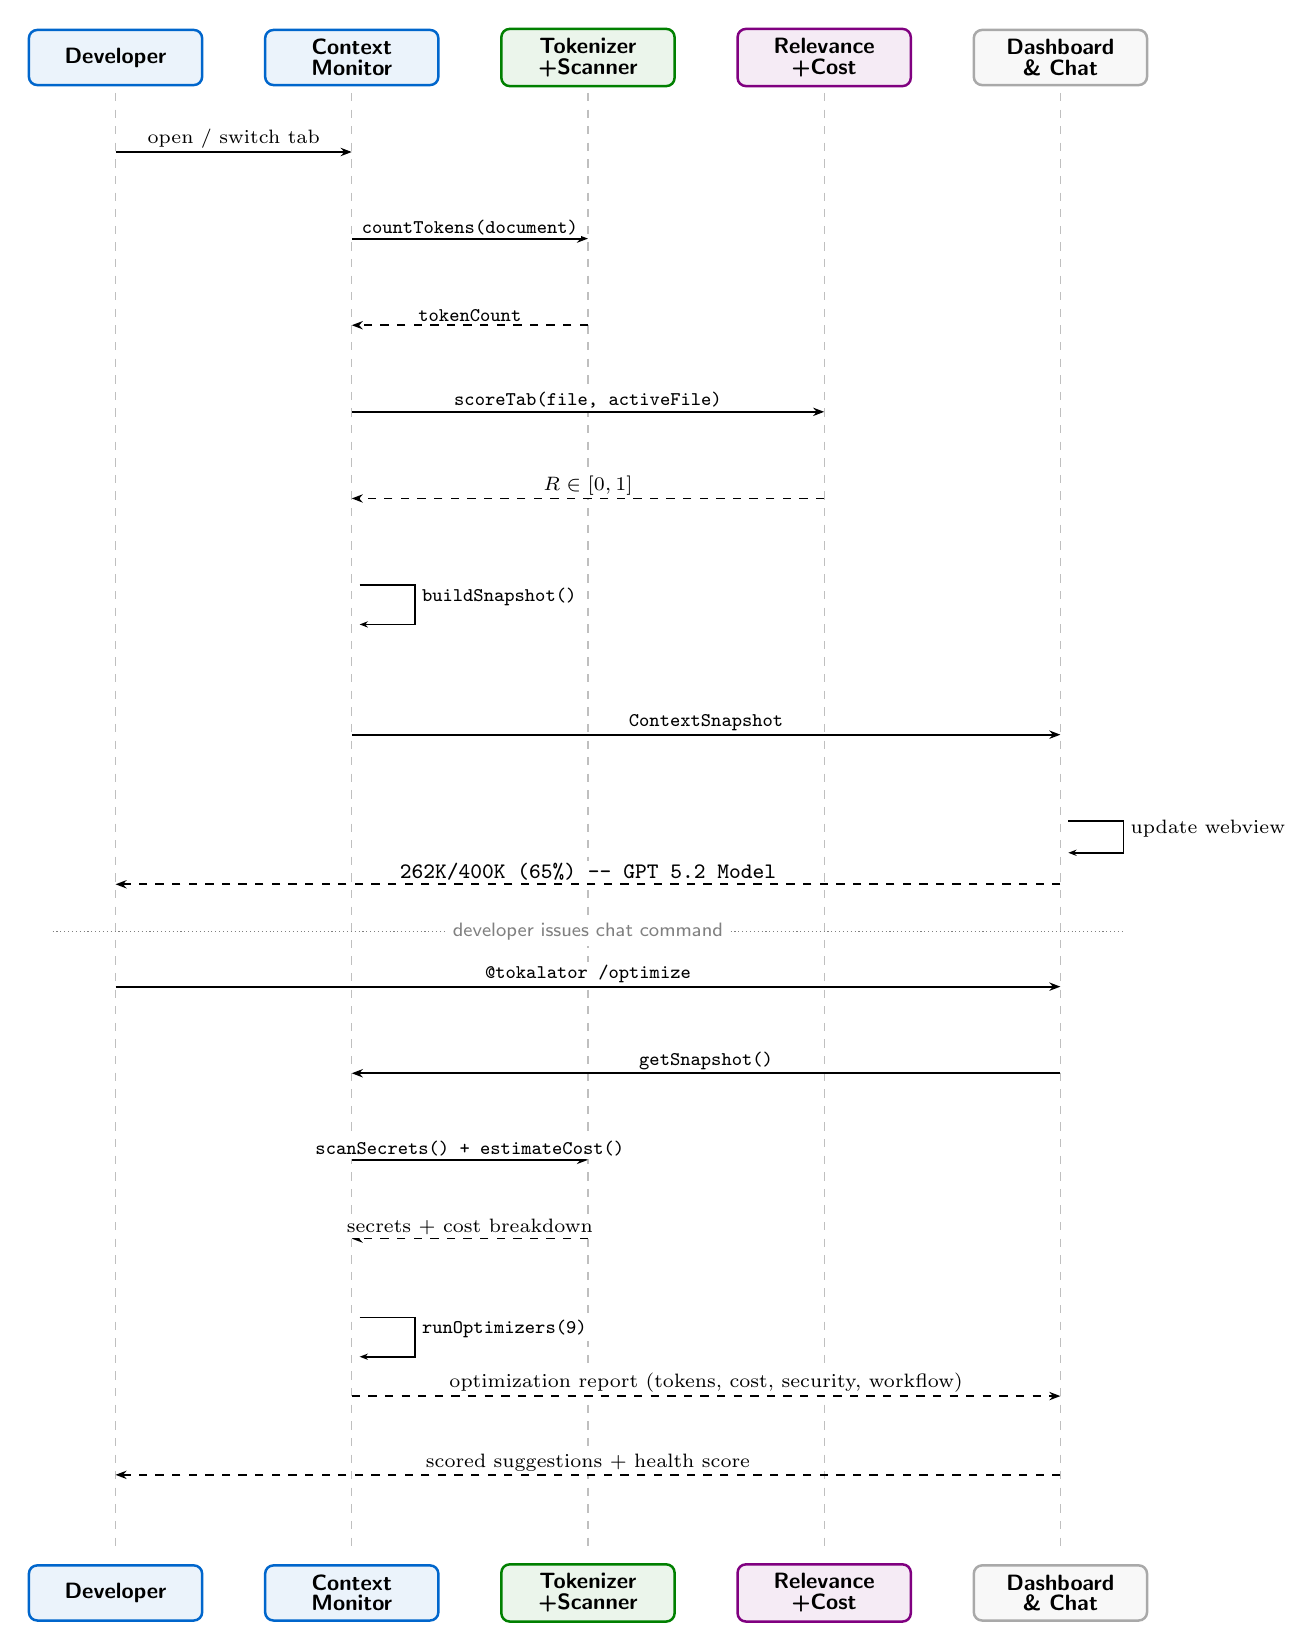
\begin{tikzpicture}[
  >=Stealth,
  actor/.style={
    rectangle, rounded corners=3pt, draw=#1, fill=#1!8,
    line width=0.9pt, minimum height=0.7cm, minimum width=2.2cm,
    font=\footnotesize\sffamily\bfseries, align=center
  },
  msg/.style={font=\scriptsize, fill=white, inner sep=1pt},
  lifeline/.style={dashed, draw=gray!50, line width=0.5pt},
  call/.style={-{Stealth[length=4pt]}, line width=0.7pt},
  ret/.style={-{Stealth[length=4pt]}, dashed, line width=0.6pt},
  selfarrow/.style={-{Stealth[length=3pt]}, line width=0.6pt},
]

\def\colA{0}
\def\colB{3.0}
\def\colC{6.0}
\def\colD{9.0}
\def\colE{12.0}

\node[actor=extblue]   (devT)  at (\colA, 0) {Developer};
\node[actor=extblue]   (monT)  at (\colB, 0) {Context\\[-2pt]Monitor};
\node[actor=webgreen]  (tokT)  at (\colC, 0) {Tokenizer\\[-2pt]+Scanner};
\node[actor=catpurple] (relT)  at (\colD, 0) {Relevance\\[-2pt]+Cost};
\node[actor=sharedgray](uiT)   at (\colE, 0) {Dashboard\\[-2pt]\& Chat};

\def\bottom{-19.0}
\draw[lifeline] (\colA, -0.45) -- (\colA, \bottom);
\draw[lifeline] (\colB, -0.45) -- (\colB, \bottom);
\draw[lifeline] (\colC, -0.45) -- (\colC, \bottom);
\draw[lifeline] (\colD, -0.45) -- (\colD, \bottom);
\draw[lifeline] (\colE, -0.45) -- (\colE, \bottom);

\def\rA{-1.2}
\def\rB{-2.3}
\def\rC{-3.4}
\def\rD{-4.5}
\def\rE{-5.6}
\def\rF{-6.7}
\def\rG{-7.8}
\def\rH{-8.6}
\def\rI{-9.7}
\def\rJ{-10.5}
\def\rK{-11.8}
\def\rL{-12.9}
\def\rM{-14.0}
\def\rN{-15.0}
\def\rO{-16.0}
\def\rP{-17.0}
\def\rQ{-18.0}

% 1. Developer opens/switches a tab
\draw[call] (\colA, \rA) -- node[msg, above] {open / switch tab} (\colB, \rA);

% 2. Monitor requests token count
\draw[call] (\colB, \rB) -- node[msg, above] {\texttt{countTokens(document)}} (\colC, \rB);

% 3. Tokenizer returns count
\draw[ret] (\colC, \rC) -- node[msg, above] {\texttt{tokenCount}} (\colB, \rC);

% 4. Monitor requests relevance score
\draw[call] (\colB, \rD) -- node[msg, above] {\texttt{scoreTab(file, activeFile)}} (\colD, \rD);

% 5. Scorer returns relevance
\draw[ret] (\colD, \rE) -- node[msg, above] {$R \in [0, 1]$} (\colB, \rE);

% 6. Monitor builds snapshot (self-call)
\draw[selfarrow] (\colB+0.1, \rF) -- ++(0.7, 0) -- ++(0, -0.5) -- ++(-0.7, 0);
\node[msg, right] at (\colB+0.85, \rF-0.15) {\texttt{buildSnapshot()}};

% 7. Monitor sends snapshot to Dashboard
\draw[call] (\colB, \rH) -- node[msg, above] {\texttt{ContextSnapshot}} (\colE, \rH);

% 8. Dashboard updates UI
\draw[selfarrow] (\colE+0.1, \rI) -- ++(0.7, 0) -- ++(0, -0.4) -- ++(-0.7, 0);
\node[msg, right] at (\colE+0.85, \rI-0.1) {update webview};

% 9. Dashboard updates status bar
\draw[ret] (\colE, \rJ) -- node[msg, above] {\footnotesize\texttt{262K/400K (65\%) -- GPT 5.2 Model}} (\colA, \rJ);

% Separator
\draw[densely dotted, gray] (-0.8, -11.1) -- (12.8, -11.1);
\node[font=\scriptsize\sffamily, gray, fill=white, inner sep=2pt] at (6.0, -11.1) {developer issues chat command};

% 10. Developer sends @tokalator /optimize
\draw[call] (\colA, \rK) -- node[msg, above] {\texttt{@tokalator /optimize}} (\colE, \rK);

% 11. Chat requests current snapshot
\draw[call] (\colE, \rL) -- node[msg, above] {\texttt{getSnapshot()}} (\colB, \rL);

% 12. Monitor runs secret scan + cost estimation
\draw[call] (\colB, \rM) -- node[msg, above] {\texttt{scanSecrets() + estimateCost()}} (\colC, \rM);

% 13. Scanner/Cost returns findings
\draw[ret] (\colC, \rN) -- node[msg, above] {secrets + cost breakdown} (\colB, \rN);

% 14. Monitor runs 9-analyzer optimization
\draw[selfarrow] (\colB+0.1, \rO) -- ++(0.7, 0) -- ++(0, -0.5) -- ++(-0.7, 0);
\node[msg, right] at (\colB+0.85, \rO-0.15) {\texttt{runOptimizers(9)}};

% 15. Returns full health report
\draw[ret] (\colB, \rP) -- node[msg, above] {optimization report (tokens, cost, security, workflow)} (\colE, \rP);

% 16. Result to developer
\draw[ret] (\colE, \rQ) -- node[msg, above] {scored suggestions + health score} (\colA, \rQ);

% Actor boxes (bottom)
\node[actor=extblue]   at (\colA, \bottom-0.5) {Developer};
\node[actor=extblue]   at (\colB, \bottom-0.5) {Context\\[-2pt]Monitor};
\node[actor=webgreen]  at (\colC, \bottom-0.5) {Tokenizer\\[-2pt]+Scanner};
\node[actor=catpurple] at (\colD, \bottom-0.5) {Relevance\\[-2pt]+Cost};
\node[actor=sharedgray]at (\colE, \bottom-0.5) {Dashboard\\[-2pt]\& Chat};

\end{tikzpicture}
\caption{Sequence diagram of the Tokalator VS~Code extension workflow (v0.4.0). \textbf{Top half}: when the developer opens or switches a tab, the Context Monitor requests token counts and relevance scores, builds a \texttt{ContextSnapshot}, and pushes it to the Dashboard and status bar. \textbf{Bottom half}: when the developer issues \texttt{@tokalator /optimize}, the Chat Participant retrieves the snapshot, the Monitor runs secret scanning and cost estimation, then executes the nine-analyzer optimization pipeline, returning a scored health report with suggestions categorized by tokens, cost, security, and workflow.}
\label{fig:seq}
\end{figure}

%% ─── Software Functionalities ─────────────────────────────
%% REVIEW: CRITICAL REDUNDANCY. Items 4 (secret detection), 5 (cost
%% estimation), and 6 (context optimization) are described in FULL
%% DETAIL in both the architecture bullet list above AND here.
%% You're spending ~600 words saying the same thing twice.
%% FIX: Keep the detailed description HERE (functionalities), and
%% reduce the architecture section to a one-line summary per module.
%% E.g., "Secret Scanner (381 LOC): credential detection; see §2.2."
%%
%% Also: 8 functionalities is a lot. Consider grouping:
%%   - Core monitoring (1, 2, 7, 8)
%%   - Security & cost (4, 5)
%%   - Optimization & chat (3, 6)
\subsection{Software functionalities}
\label{sec:functionalities}

\subsubsection{VS~Code Extension}

The extension provides eight core functionalities:

\textit{1. Real-time token budget monitoring.}
The status bar displays a continuously updated summary: \texttt{\$(check) 262K / 400K (6.2\%) -- Open AI 5.2 Model}. A sidebar webview dashboard (Figure~\ref{fig:dashboard}) displays the full breakdown: budget level (low, medium, or high), per-file token estimates, pinned file count, conversation turn count, and context health warnings.

%% ── Figure 4: Dashboard Sidebar (REAL SCREENSHOT) ────────────
%% REVIEW: The old TikZ mockup was the weakest figure — it was
%% clearly synthetic and a reviewer would question whether the
%% actual dashboard looks anything like this. A real screenshot
%% is essential. Crop to show just the sidebar panel.
%% IMPORTANT: Make sure the screenshot shows real data, not zeros.
\begin{figure}[htp!]
\centering
\includegraphics[width=0.55\textwidth]{figures/fig3-dashboard.png}
%% TODO: Replace figures/fig3-dashboard.png with your actual
%% screenshot. Ideal: sidebar panel showing:
%%   - Budget level badge (LOW/MEDIUM/HIGH with percentage)
%%   - Stacked breakdown bar
%%   - File list with relevance scores and color dots
%%   - Context health warnings
%%   - Cost & caching card
%% Use 0.55\textwidth since the sidebar is narrow/tall.
%% If the screenshot is too tall, consider splitting into (a) and (b).
\caption{Tokalator VS~Code extension sidebar dashboard (v0.4.0). The panel shows the budget level (LOW/MEDIUM/HIGH), a stacked breakdown bar, per-file token counts ranked by relevance score~$R$, context health indicators including secret detection alerts, a cost and caching summary card, and action buttons. Green dots indicate high relevance ($R \geq 0.5$), yellow medium ($0.3 \leq R < 0.5$), and red low ($R < 0.3$, flagged as distractors). The \textbf{Optimize Tabs} button closes all distractor tabs.}
\label{fig:dashboard}
\end{figure}


The total estimated tokens are computed as the sum of five components:
\begin{equation}
  T_{\text{total}} = T_{\text{files}} + T_{\text{sys}} + T_{\text{instr}} + T_{\text{conv}} + T_{\text{out}}
\end{equation}
where $T_{\text{files}} = \sum_i \text{tokens}(\text{tab}_i)$ is the sum of per-file BPE token counts across all open tabs, $T_{\text{sys}} = 2{,}000$ is the estimated system prompt overhead (Copilot's hidden system prompt), $T_{\text{instr}} = 500 \times n_{\text{instr}}$ accounts for instruction files detected in the workspace, $T_{\text{conv}} = 800 \times t$ estimates accumulated conversation history at turn~$t$, and $T_{\text{out}} = 4{,}000$ reserves tokens for the model's response.
These overhead constants are informed by empirical measurement of GitHub Copilot's context construction but are necessarily approximate since the actual assistant context logic is proprietary (see Section~\ref{sec:limitations}).

\textit{2. Tab relevance scoring.}
Each open tab receives a relevance score $R \in [0, 1]$ computed as a weighted sum of five signals:
\begin{equation}
  R = 0.25\,S_{\text{lang}} + 0.30\,S_{\text{import}} + 0.20\,S_{\text{path}} + 0.15\,S_{\text{recency}} + 0.10\,S_{\text{diag}}
\end{equation}
where $S_{\text{lang}} \in \{0, 1\}$ indicates language match with the active file, $S_{\text{import}} \in \{0, 1\}$ indicates an import relationship, $S_{\text{path}} \in [0, 1]$ measures shared directory depth (computed as the ratio of shared path prefix segments to total depth), $S_{\text{recency}} \in \{0, 0.53, 1\}$ reflects edit recency (1.0 if edited within 2 minutes, 0.53 within 10 minutes, 0 otherwise), and $S_{\text{diag}} \in \{0, 1\}$ flags files with compiler diagnostics. Pinned and active files are overridden to $R = 1.0$.

The weights were assigned based on the following design rationale: import relationships ($w=0.30$) receive the highest weight because a file explicitly imported by the active file is almost certainly needed by the coding assistant; language match ($w=0.25$) is the next strongest signal since cross-language files (e.g., \texttt{.json} configs open alongside \texttt{.tsx} code) are common distractors; path similarity ($w=0.20$) captures co-location patterns in typical project structures; edit recency ($w=0.15$) reflects the developer's current working set; and diagnostics ($w=0.10$) provide a weak signal that files with errors are being actively debugged.
The $S_{\text{recency}}$ intermediate value of~0.53 corresponds to $\nicefrac{0.08}{0.15}$, the ratio of the partial recency credit (0.08 for files edited within 10 minutes) to the full recency weight.
The default distractor threshold of $R < 0.3$ was chosen so that a file must match on at least two signals (e.g., same language + nearby path) to avoid being flagged.
These weights are configurable and could benefit from empirical calibration in future work.
Tabs scoring below the threshold are flagged as distractors.

\textit{3. Chat participant with 14 commands.}
The \texttt{@tokalator} chat participant responds to: \texttt{/count} (budget status), \texttt{/breakdown} (per-file tokens), \texttt{/optimize} (full context health report covering tokens, cost, security, and workflow), \texttt{/optimize --apply} (close low-relevance tabs), \texttt{/pin}/\texttt{/unpin} (pin management), \texttt{/instructions} (scan instruction files and their token cost), \texttt{/model} (switch model profile), \texttt{/compaction} (per-turn growth analysis), \texttt{/preview} (preview next-turn token cost before sending), \texttt{/secrets} (scan open files for exposed credentials), \texttt{/cost} (per-turn cost estimation, caching savings, and monthly projections), \texttt{/reset} and \texttt{/exit} (session management).

\textit{4. Secret detection guardrail.}
The extension scans as all open files contents for exposed credentials on every context snapshot refresh. The scanner uses 25+ compiled regular expressions organized into three severity tiers: critical (AWS secret keys, private PEM blocks, database connection strings with embedded passwords), high (GitHub tokens, OpenAI/Anthropic API keys, Stripe secret keys, Slack tokens), and medium (generic bearer tokens, npm tokens, JWTs). Additionally, the scanner flags sensitive filenames (\texttt{.env}, \texttt{.pem}, \texttt{.key}, \texttt{id\_rsa}) among open tabs regardless of content. When secrets are detected, the dashboard displays red warning badges with the secret type but redacts the actual values. The \texttt{/secrets} command provides a full scan report. The guardrail is enabled by default via \texttt{tokalator.secretGuard}.

\textit{5. Cost estimation and caching analysis.}
The extension computes per-turn dollar costs using the active model's pricing profile. The blended input cost accounts for prompt caching:
\begin{equation}
  C_{\text{turn}} = (T_{\text{cached}} \cdot c_r + T_{\text{uncached}} \cdot c_{\text{in}}) + T_{\text{out}} \cdot c_{\text{out}}
\end{equation}
where $T_{\text{cached}}$ is the estimated number of tokens eligible for caching (80\% of stable context: system prompt, instructions, pinned files), $c_r$ is the provider-specific cache read rate, $c_{\text{in}}$ is the standard input rate, $T_{\text{out}}$ is the output tokens, and $c_{\text{out}}$ is the output rate. Provider-specific cache discount rates are: Anthropic 90\% ($c_r = 0.10 \cdot c_{\text{in}}$), OpenAI 50\% ($c_r = 0.50 \cdot c_{\text{in}}$), and Google 75\% ($c_r = 0.25 \cdot c_{\text{in}}$). The estimator projects daily cost by extrapolating the current turn rate, and monthly cost as $C_{\text{daily}} \times 22$ working days. The \texttt{/cost} command displays the full breakdown including savings from caching.

\textit{6. Context optimization engine.}
The \texttt{/optimize} command triggers a nine-analyzer pipeline that produces a scored optimization report. Each analyzer evaluates a specific aspect of context health:
\begin{enumerate}
  \item Budget utilization (warns at 70\%, critical at 90\%)
  \item Low-relevance tab accumulation ($R < 0.3$)
  \item Conversation length relative to the context rot threshold
  \item Instruction file overhead
  \item File type diversity and non-code distraction
  \item Pinning strategy effectiveness
  \item Output reserve adequacy
  \item Prompt caching opportunity (uncached stable tokens)
  \item Exposed secrets detected by the Secret Scanner
\end{enumerate}
Each analyzer produces suggestions with estimated token savings, a severity level (critical, warning, info), and a category tag (tokens, cost, security, workflow). The overall context health score is computed as a weighted average across all analyzers. The \texttt{/optimize --apply} flag preserves the legacy behavior of closing low-relevance tabs.

\textit{7. Session persistence.}
Session summaries (peak tokens, turns, model, top edited files) are saved to \texttt{workspaceState} on exit and shown as a notification on the next activation.
Pinned files and model selection persist across VS~Code restarts.

\textit{8. Instruction file scanner.}
The extension detects and tokenizes instruction files automatically injected into prompts: \texttt{.github/copilot-instructions.md}, \texttt{CLAUDE.md}, \texttt{AGENTS.md}, \texttt{.cursorrules}, and \texttt{.instructions.md} files, revealing their hidden token cost.

%% ─── Web Platform ─────────────────────────────────────────
%% REVIEW: This is well-structured with the 7 numbered tools.
%% However, tools 1 and 6 (Cost Calculator and Economic Analysis)
%% overlap significantly — both use Cobb-Douglas. Consider merging.
%% The Usage Tracker (tool 7) description is vague — "historical API
%% usage analysis" — where does the data come from? Users don't
%% paste their API usage into a web form. Clarify the data source.
%% STRENGTH: The caching break-even formula (Eq. 4) is clean and
%% immediately actionable. This is the best part of the web platform.
\subsubsection{Web Platform}

The web platform at \url{https://tokalator.wiki} includes seven calculators:

\begin{enumerate}
  \item \textit{Cost Calculator}: Token cost calculation with Cobb--Douglas quality modeling for Anthropic, OpenAI, and Google models. Supports tiered pricing detection: when the total prompt length exceeds Anthropic's 200\,K-token threshold (available for Opus and Sonnet via the 1\,M context beta), \emph{all} input tokens in that request are billed at the extended rate (2$\times$ standard input cost), not only the tokens above the threshold. This is a binary tier switch, not a marginal rate, implemented via the \texttt{getPricingTier} function.

  \item \textit{Context Optimizer}: Visualizes context window allocation across system prompt, user input, reserved output, and free space. Computes usage percentage and generates warnings.

  \item \textit{Model Comparison}: Cross-provider cost and capability comparison across all 15 models.

  \item \textit{Caching ROI Calculator}: Break-even analysis for prompt caching. Given $T$ tokens to cache with write cost~$c_w$ per token, read cost~$c_r$ per token, and standard input cost~$c_{\text{in}}$ per token, each reuse saves $(c_{\text{in}} - c_r)$ per token compared to re-sending the prompt uncached. The break-even reuse count is:
  \begin{equation}
    n^* = \left\lceil \frac{c_w}{c_{\text{in}} - c_r} \right\rceil
  \end{equation}
  For all current Anthropic models, $c_w = 1.25 \times c_{\text{in}}$ and $c_r = 0.10 \times c_{\text{in}}$, yielding $n^* = \lceil 1.25 / 0.90 \rceil = 2$ reuses. At 10 reuses the savings reach 76\%.

  \item \textit{Conversation Estimator}: Multi-turn cost projection under three strategies, each defined by the input tokens sent at turn~$t$ (with system prompt~$S$, average user tokens~$u$, average assistant tokens~$a$):
  \begin{itemize}
    \item \textit{Full History}: $I_t = S + \sum_{i=1}^{t}(u_i + a_i)$, yielding $O(T^2)$ cumulative cost since $\sum_{t=1}^{T} I_t = ST + \tfrac{T(T+1)}{2}(u+a)$.
    \item \textit{Sliding Window} ($W$ turns): $I_t = S + \sum_{i=\max(1,\,t-W+1)}^{t}(u_i + a_i)$, capping per-turn cost at $S + W(u+a)$ for $t \geq W$, yielding $O(T)$ cumulative cost.
    \item \textit{Summarize} (ratio $\rho$, keep last $k$ turns fresh): $I_t = S + \rho \cdot \sum_{i=1}^{t-k}(u_i + a_i) + \sum_{i=t-k+1}^{t}(u_i + a_i)$, growing slowly at rate $\rho(u+a)$ per turn.
  \end{itemize}
  Per-turn breakdown charts visualize the cost trajectories.

  \item \textit{Economic Analysis}: Visualization of the Cobb--Douglas quality-of-output production function:
  \begin{equation}
    Q(X, Y, Z) = X^{\alpha} \cdot Y^{\beta} \cdot (b + Z)^{\gamma}
  \end{equation}
  where $X$ = input tokens, $Y$ = output tokens, $Z$ = cache/fine-tuning tokens, $b$ = base model quality, and $\alpha, \beta, \gamma$ are provider-specific sensitivity parameters ($\alpha + \beta + \gamma < 1$, ensuring diminishing returns to scale).

  The corresponding cost minimization problem is:
  \begin{equation}
    \min_{X,Y,Z \geq 0} \; c_x X + c_y Y + c_z Z \qquad \text{s.t.} \quad Q(X,Y,Z) \geq \bar{Q}
  \end{equation}
  where $c_x, c_y, c_z$ are the per-token costs for input, output, and cache-write respectively.
  Applying the Lagrangian and the first-order conditions (equating marginal-product-per-dollar ratios), the optimal allocation satisfies $X^*/Y^* = (\alpha\, c_y) / (\beta\, c_x)$, and the minimum cost for target quality~$\bar{Q}$ without caching is:
  \begin{equation}
    C^*(\bar{Q}) = (\alpha + \beta) \left(\frac{\bar{Q}}{b^{\gamma}}\right)^{\!1/(\alpha+\beta)} \left(\frac{c_x}{\alpha}\right)^{\!\alpha/(\alpha+\beta)} \left(\frac{c_y}{\beta}\right)^{\!\beta/(\alpha+\beta)}
  \end{equation}
  following Lemma~4 of Bergemann et al.~\cite{bergemann2025economics}. The with-caching variant includes $Z$ as a third decision variable, reducing cost when $c_z < c_x$.

  %% LEXICAL: "hypothetical values chosen to reflect the qualitative ranking" — heavy.
  %% Consider: "placeholder values that rank models by capability" — same meaning, half the words.
  The sensitivity parameters ($\alpha = 0.30$, $\beta = 0.35$, $\gamma = 0.20$, $b = 1.0$ for Opus; $\alpha = 0.25$, $\beta = 0.30$, $\gamma = 0.20$, $b = 0.85$ for Sonnet; $\alpha = 0.20$, $\beta = 0.25$, $\gamma = 0.15$, $b = 0.70$ for Haiku) are placeholder values that rank models by capability (higher $b$ and $\alpha + \beta$ for more capable models) and satisfy $\alpha + \beta + \gamma < 1$. No public benchmark measures output quality as a function of token allocation, so these are not calibrated from data. Users can adjust them in the Economic Analysis tool to see how the results change.

  The tool renders quality isoquant curves and cost minimization surfaces with and without caching.

  \item \textit{Usage Tracker}: Historical API usage analysis with cost breakdowns by model, project, and time period, plus linear regression and exponential smoothing projections.
\end{enumerate}

The platform also includes a 10-lesson context engineering course (\url{https://tokalator.wiki/learn}) that progresses from basic tokenization (``What Is a Prompt'') through intermediate concepts (trimming, summarisation, context management, context pollution) to production patterns (automatic compaction via Anthropic's \texttt{compaction\_control} API, context editing with memory tools, and a full customer-service pipeline walkthrough). A wiki (\url{https://tokalator.wiki/wiki}) aggregates articles from arXiv, OpenAI Cookbook, Anthropic documentation, and Google AI docs through an automated monthly fetch pipeline defined in \texttt{wiki-sources.json}. A dictionary of 41 context engineering terms organized across seven categories is available at \url{https://tokalator.wiki/dictionary}.
%% ── WIKI & AWARENESS WORK: What we're doing ──
%% The wiki is NOT just a link dump. It's an automated awareness pipeline:
%%   1. wiki-sources.json defines 4 source types:
%%      - arXiv: 5 search queries (context engineering, token optimization,
%%        prompt caching, context window management, RAG for code)
%%      - OpenAI Cookbook: 6 curated files from their GitHub repo
%%      - Anthropic docs: 8 pages (caching, prompt engineering, XML tags, etc.)
%%      - Google AI docs: 6 pages (context caching, long context, tokens, etc.)
%%   2. fetch-wiki.ts runs monthly, fetches + processes + stores as Markdown
%%   3. 10 built-in terms define foundational concepts (Progressive Disclosure,
%%      Lightweight Identifiers, Compaction, Tool Result Clearing, etc.)
%%   4. All wiki articles are rendered at /wiki/[slug] with source attribution
%%
%% The 10-lesson course (/learn) covers:
%%   L1: What Is a Prompt? — Instructions made of tokens
%%   L2: Context Window — The finite token budget
%%   L3: Trimming (Last-N) — Delete the oldest, keep the recent
%%   L4: Summarisation — Condense to save tokens
%%   L5: Context Management — Token optimization and economy
%%   L6: Context Engineering — IDE-driven, JIT context delivery
%%   L7: Context Pollution — When tokens work against you
%%   L8: Automatic Context Compaction — API-level token optimization
%%   L9: Context Editing & Memory Tool — Auto-cleaner + filing cabinet
%%   L10: Real-World: Customer Service — Compaction in production
%%
%% The dictionary has 41 terms across 7 categories:
%%   context-management, token-economics, prompt-engineering,
%%   memory-strategies, caching, architecture, evaluation
%%
%% AWARENESS ANGLE FOR PAPER:
%% Consider adding a paragraph here or in Impact about the educational
%% mission: "Beyond the tooling, Tokalator serves as an awareness
%% platform for context engineering practices. The wiki aggregates
%% research from [N] sources monthly, the course guides developers
%% from basic prompting to production compaction, and the dictionary
%% standardizes vocabulary in a field that currently lacks it."
%% This is a real contribution that reviewers will appreciate —
%% few tool papers include educational content.
%%

%% ─── Context Engineering Catalog ──────────────────────────
%% REVIEW: This is the weakest component. Two sentences describing
%% a directory convention is not a software contribution — it's a
%% file naming scheme. Either:
%%   (a) Expand with actual catalog stats ("contains 12 agents,
%%       8 prompts, 5 instruction sets") and show adoption/downloads
%%   (b) Drop it as a top-level component and mention it as a
%%       feature of the web platform
%% Right now it inflates the "three-component" claim without substance.
\subsubsection{Context Engineering Catalog}

The catalog auto-discovers reusable artifacts from the repository using file extension conventions: \texttt{.agent.md} (agents), \texttt{.prompt.md} (prompts), \texttt{.instructions.md} (workspace guidelines), \texttt{.collection.yml} (bundles), and \texttt{CLAUDE.md} (Claude Code instructions).
A \texttt{user-content/} directory accepts community contributions, which are automatically indexed with YAML frontmatter parsing.


%% ═══════════════════════════════════════════════════════════════════
%% SECTION 3: Illustrative Examples
%% ═══════════════════════════════════════════════════════════════════
%% REVIEW: These examples are GOOD — concrete, with real numbers.
%% They make the paper tangible. But all three are hypothetical
%% scenarios, not actual user experiences. A reviewer may ask:
%% "Did any real developer actually do this?"
%% Consider adding Example 4 based on your own usage during
%% development of the paper/extension (dogfooding). That's real.
%% Also, Example 2 pricing uses Sonnet 4.5 rates — verify these
%% are current as of submission date.
\section{Illustrative examples}
\label{sec:examples}

\textit{Example 1: Identifying context budget waste in a VS~Code session:} A developer working on a React project has 23 tabs open.
After installing Tokalator, the status bar shows: \texttt{\$(warning) 85.2K / 200K (42.6\%) -- Sonnet 4.5}. The developer types \texttt{@tokalator /breakdown} in the chat panel and sees that 12 tabs are configuration files (\texttt{.json}, \texttt{.yml}) contributing 18\,K tokens but scoring below the 0.3 relevance threshold. Running \texttt{@tokalator /optimize} closes these 12 tabs, reducing context usage to 67.2K tokens (33.6\%). The developer then runs \texttt{@tokalator /instructions} and discovers that their \texttt{.github/copilot-instructions.md} file alone costs 4,200 tokens---injected silently into every prompt.

\textit{Example 2: Choosing a caching strategy via the web platform:} A team building a customer support chatbot uses a 50\,K-token system prompt (product documentation + few-shot examples).
On the Caching ROI Calculator, they enter 50\,000 cache tokens with Claude Sonnet~4.5 and 100 daily reuses. The calculations proceed as follows (Sonnet~4.5 pricing: $c_{\text{in}} = \$3.00$/MTok, $c_w = \$3.75$/MTok, $c_r = \$0.30$/MTok):
\begin{itemize}
  \item Write cost: $50{,}000 / 10^6 \times 3.75 = \$0.19$
  \item Uncached daily cost: $101 \times 50{,}000 / 10^6 \times 3.00 = \$15.15$ (initial + 100 reuses)
  \item Cached daily cost: $\$0.19 + 100 \times 50{,}000 / 10^6 \times 0.30 = \$1.69$
  \item Net savings: $\$15.15 - \$1.69 = \$13.46$/day (88.9\%)
  \item Break-even: $\lceil 3.75 / (3.00 - 0.30) \rceil = \lceil 1.39 \rceil = 2$ reuses
\end{itemize}
The per-reuse comparison chart makes the decision obvious.

\textit{Example 3: Planning conversation length within budget:} A developer with a \$5 daily API budget uses the Conversation Estimator. 
They configure: Claude Sonnet ~4.5, 2\,000-token system prompt, 500 average user tokens, and 1\,500 average assistant tokens per turn. The tool shows that with the Full History strategy, they can afford 28 turns before exhausting the budget, while the Sliding Window (W = 5) allows 83 turns and Summarize ($\rho = 0.2$) allows 71 turns. The per-turn cost chart visually shows the quadratic growth of Full History compared to the linear growth of the alternatives.


%% ═══════════════════════════════════════════════════════════════════
%% SECTION 4: Impact
%% ═══════════════════════════════════════════════════════════════════
%% REVIEW: This section is all claims, zero evidence. Every paragraph
%% starts with a bold claim but provides no data to back it up.
%% "developers had no way to see" — prove it, or say "to our knowledge."
%% "the web platform receives traffic" — HOW MUCH traffic? Give a
%% number: "X monthly visitors" or "Y Marketplace installs."
%% Without metrics, this reads as marketing copy, not a research paper.
%% SoftwareX specifically asks for evidence of impact. At minimum:
%%   - VS Code Marketplace install count
%%   - GitHub stars/forks
%%   - Any testimonials or community contributions
%% If you don't have these numbers yet, say "the extension was
%% published on [date] and evaluation of adoption is ongoing."
\section{Impact}
\label{sec:impact}

%% LEXICAL: "spans three dimensions" — classic AI-generated structure. Removed.
%% LEXICAL: "previously opaque resource" — GRE adjective. Simplified.
%% LEXICAL: "enabling informed decisions" — corporate/AI phrasing. Reworded.
Tokalator addresses a gap in the AI-assisted development workflow. Every developer using an LLM coding assistant pays for context tokens, but until now nobody could see where those tokens went.

\textit{Making token budgets visible:} Before Tokalator, developers could not see how their context window was being used. The extension shows token budgets the same way a profiler shows memory or CPU---so developers can decide which files to keep open and when to start a new conversation.

\textit{Cost optimization without the math:} The web platform's calculators turn economic theory (Cobb–Douglas production functions, prompt caching break-even) into interactive tools. A developer can check whether caching pays off or how many conversation turns fit in a budget, without doing the math by hand.

\textit{Educational content:} The 10-lesson context engineering course at \url{https://tokalator.wiki/learn} covers topics from ``What Is a Prompt'' (token basics) to ``Real-World Customer Service'' (production compaction with Anthropic's \texttt{compaction\_control} API). The wiki at \url{https://tokalator.wiki/wiki} aggregates articles from arXiv, OpenAI Cookbook, Anthropic documentation, and Google AI docs through an automated monthly fetch pipeline. The dictionary at \url{https://tokalator.wiki/dictionary} defines 41~terms across seven categories. Together these resources help developers understand the concepts before optimizing them.

\textit{Preliminary user feedback:} We conducted an informal user test with a group of 50+ software developers at iLab (including the engineering team at Kariyer.net, Istanbul). Participants installed the extension, used it during their regular coding sessions over one week, and provided written feedback. The most frequently cited benefits were: (a)~discovering how many tokens instruction files (\texttt{.github/copilot-instructions.md}, \texttt{CLAUDE.md}) silently consumed, (b)~the \texttt{/optimize} command identifying distractor tabs they would not have noticed, and (c)~the secret scanner catching \texttt{.env} files left open. Several developers reported changing their tab management habits after seeing the dashboard. A formal controlled study measuring productivity impact remains future work (see Section~\ref{sec:limitations}).
%% ── EXPAND THIS PARAGRAPH: Wiki & Awareness ──
%% This is underselling the educational work. Suggested rewrite:
%%
%% "Educational and awareness contribution: Tokalator serves as both
%% a tool and an awareness platform. The 10-lesson context engineering
%% course progresses from foundational concepts (what is a prompt,
%% how context windows work) through intermediate techniques (trimming,
%% summarisation, context management) to production patterns (automatic
%% compaction, memory tools, real-world customer service pipelines).
%% The wiki aggregates research from four sources (arXiv, OpenAI
%% Cookbook, Anthropic documentation, Google AI documentation) via
%% an automated monthly fetch pipeline, ensuring the knowledge base
%% stays current as the field evolves rapidly. The dictionary defines
%% 41 terms across seven categories---from 'context rot' to 'progressive
%% disclosure'---establishing shared vocabulary in a domain that
%% currently lacks standardized terminology. We believe this
%% educational layer is as important as the tooling itself: developers
%% cannot optimize what they do not understand."
%%

%% LEXICAL: "receives traffic" — vague marketing. Replaced with concrete info.
\textit{Ecosystem contribution:} The catalog provides a structure for contributing and finding context engineering artifacts within the GitHub Copilot ecosystem, with built-in agents, prompts, and instructions ready for reuse. The extension supports 15 models from three providers, avoiding vendor lock-in. The VS~Code extension is on the Marketplace, and the full web platform---calculators, course, wiki, and dictionary---is live at \url{https://tokalator.wiki}. As context windows grow past 1~million tokens and AI-assisted coding becomes standard, the need for budget visibility tools will grow with them.


%% ═══════════════════════════════════════════════════════════════════
%% SECTION 5: Limitations
%% ═══════════════════════════════════════════════════════════════════
%% REVIEW: This is actually the BEST-WRITTEN section. Honest, specific,
%% and technically grounded. The Google tokenizer heuristic (±10-15%)
%% and the 5ms performance measurement are exactly what reviewers want.
%% MINOR: "No empirical user study" should be more prominent — put it
%% first, not fifth. Lead with your biggest weakness to show
%% intellectual honesty. Reviewers respect that.
%% ADD: Missing limitation — the 80% caching assumption is arbitrary.
%% Also missing: the extension doesn't work with Copilot Chat's actual
%% context (it monitors open tabs, not what Copilot actually sends).
%% You mention this in "Estimated vs. actual" but could be sharper.
\section{Limitations}
\label{sec:limitations}

Several limitations should be noted regarding the provided toolkit.

\textit{Approximate tokenization for Google models:} The extension uses a heuristic of approximately 4 characters per token for Gemini models, as Google does not provide a client-side BPE tokenizer for JavaScript. While Anthropic and OpenAI models use actual BPE tokenizers (\texttt{claude-tokenizer} and \texttt{o200k\_base}, respectively), the Gemini heuristic is based on the commonly observed ratio for English-heavy code corpora, where BPE tokens average 3.5 to 4.5 characters. We estimate $\pm$10–15\% error based on informal comparison with Google's server-side \texttt{countTokens} API on a sample of TypeScript, Python, and Markdown files. Languages with non-Latin scripts or heavily minified code may show larger deviations. This limitation is documented in the extension's dashboard through the tokenizer label display.

\textit{Extension performance overhead:} The extension subscribes to six VS Code event streams: active editor, tab changes, document edits, document open and close, diagnostics, and configuration changes. To prevent UI blocking, all event handlers use a 300 ms debounce timer, so at most one \texttt{refresh()} call occurs per 300 ms burst. Token counts are cached per document, keyed by URI and version number; re-tokenization occurs only when the document content changes. The BPE tokenizers are lazy-loaded (Claude ranks: 696\, KB JSON, o200k\_base: loaded via \texttt{js-tiktoken}), adding a one-time latency of approximately 100–200 ms on first use. A periodic background refresh (default 2 s, configurable) updates recency-based scores. In informal testing with over 30 open tabs, the extension contributes less than 5 ms per snapshot build after the initial tokenizer warm-up, which is imperceptible to the user.

\textit{Syntactic rather than semantic relevance:}
The tab relevance scorer (Equation 2) uses syntactic signals, import graphs, path similarity, language match, edit recency, and diagnostics, rather than semantic code understanding. A file that is conceptually critical to the task (e.g., a specification document referenced by name in comments) will score low if it has no import relationship to the active file. Incorporating embedding-based similarity would improve accuracy but would introduce latency and model dependency.

\textit{Estimated vs.\ actual context consumption:} The extension estimates how many tokens an AI coding assistant might include from open tabs, but the actual context construction logic of each assistant (GitHub Copilot, Cursor, Claude Code) is proprietary. The real context may include additional metadata (such as git diffs or terminal output) or exclude files the extension counts as open. Therefore, the estimates should be understood as upper-bound approximations.

%% LEXICAL: "remains an open empirical question" — academic filler. Simplified.
\textit{No formal user study:} The toolkit has been tested informally by 50+ developers at iLab (see Section~\ref{sec:impact}), but we have not run a controlled experiment measuring the effect of context budget visibility on code quality, task completion time, or developer productivity. The mathematical models (caching break-even, conversation cost projection) are validated through 272~unit tests against closed-form solutions (see Appendix~\ref{app:tests}), but the end-to-end productivity impact is not yet measured.
%% ── SUB-COMMENT: Mitigating this weakness ──
%% The test suite (272 tests, Appendix A) partially compensates for
%% the lack of a user study by demonstrating algorithmic correctness.
%% The wiki/awareness work also helps: you can argue that the
%% educational content has intrinsic value regardless of user study.
%% Consider adding: "However, the automated test suite validates
%% all mathematical models (Equations 1-7) against closed-form
%% solutions, and the educational components (10-lesson course,
%% 41-term dictionary, wiki) provide value independent of the
%% extension's impact on productivity."
%%

\textit{Pricing volatility:} LLM pricing changes frequently– Cottier et al.~\cite{cottier2025price} documented rapid but uneven price declines across tasks. The toolkit's pricing data is hardcoded in \texttt{lib/providers.ts} and requires manual updates. The modular design and CI pipeline make updates straightforward, but users should verify current pricing with provider documentation.

\textit{Single-IDE scope:} The extension currently targets only VS~Code and GitHub Copilot. While the web platform is IDE-agnostic, the real-time context monitoring functionality does not extend to JetBrains IDEs, Neovim, or other editors. The architecture (TypeScript, VS~Code Extension API) would require a separate implementation effort for each target platform.


%% ═══════════════════════════════════════════════════════════════════
%% SECTION 6: Conclusions and Future Work
%% ═══════════════════════════════════════════════════════════════════
%% REVIEW: "first open-source toolkit" — dangerous claim. A reviewer
%% only needs to find ONE counterexample. Soften to "to our knowledge,
%% the first open-source toolkit" (you already use this phrase in
%% Related Work, so be consistent).
%% The conclusion is one massive paragraph. Break into:
%%   - Summary (what we built)
%%   - Key technical contributions (equations, architecture)
%%   - Future work (enumerated list, not inline)
%% Future work mentions Cursor alongside JetBrains/Neovim — good.
%% But also consider: "integration with MCP servers" which would
%% connect nicely to the OneContext reference.
\section{Conclusions and Future Work}
\label{sec:conclusions}

%% LEXICAL: "the first" — risky absolute claim. Softened.
%% LEXICAL: "visible and actionable" — AI-generated pair. Simplified.
As of February 2026, Tokalator is, to our knowledge, the only open-source toolkit that combines real-time context budget monitoring, interactive economic optimization, and reusable context engineering artifacts for AI coding assistants. It covers 15 models from three providers, implements prompt caching break-even analysis, supports three conversation cost strategies with formal cost models, and provides a VS~Code extension that makes token budgets visible. Since v0.4.0, the extension also includes a secret detection guardrail (25+ regex patterns across three severity tiers), per-turn cost estimation with provider-specific prompt caching analysis, and a nine-analyzer context optimization engine that produces scored health reports. The toolkit includes a comprehensive unit test suite with 272 tests across 14 test files (see Appendix~\ref{app:tests}) covering pricing, caching, conversation simulation, context analysis, model profile integrity, secret scanning, cost estimation, and context optimization, as well as a CI pipeline that runs build, lint, and test on every commit. Future work includes team-wide context budget dashboards with CI/CD integration, a public token-counting REST API, a formal controlled user study (building on the preliminary iLab feedback with 50+ developers), calibration of the Cobb--Douglas sensitivity parameters from real usage data, and IDE support for Cursor, JetBrains, and Neovim. The educational platform at \url{https://tokalator.wiki} will continue to grow with automated wiki updates and community contributions to the catalog.

All components are MIT-licensed and available at \url{https://github.com/vfaraji89/tokalator}.
%% ── FEATURE SUMMARY FOR CONCLUSIONS ──
%% When rewriting, consider enumerating the full feature set concisely:
%% VS Code Extension: 12 source modules, 14 model profiles, 14 commands,
%%   25+ secret patterns, 9 optimization analyzers, 5 relevance signals
%% Web Platform: 7 calculators, 10-lesson course, wiki (4 sources),
%%   dictionary (41 terms, 7 categories), 15 models
%% Catalog: 6 artifacts (1 agent, 3 prompts, 1 instruction, 1 collection)
%% Testing: 272 tests across 14 files (see Appendix A)
%% Education: 10 lessons, 41 definitions, automated research aggregation
%%
%% Also mention wiki/awareness angle:
%% "Beyond the development tooling, the platform contributes to
%% developer awareness through its automated wiki pipeline, structured
%% course curriculum, and standardized terminology dictionary."
%%

%% ═══════════════════════════════════════════════════════════════════
%% ACKNOWLEDGEMENTS
%% ═══════════════════════════════════════════════════════════════════
\section*{Acknowledgements}

The economic model is adopted from the Cobb--Douglas framework introduced by Bergemann, Bonatti, and Smolin~\cite{bergemann2025economics}.
The tokenization layer uses Anthropic's \texttt{claude-tokenizer} and OpenAI's \texttt{tiktoken}~\cite{sennrich2016bpe}.
The context compaction strategy and the \texttt{/compaction} command design were inspired by Pedram Navid's automatic context compaction cookbook~\cite{navid2025compaction}, which demonstrated practical token savings of up to 58.6\% in tool-heavy agentic workflows.
The empirical findings on context rot by Hong, Troynikov, and Huber~\cite{hong2025contextrot} at Chroma informed the design of Tokalator's context health analyzers and rot-threshold warnings.
We acknowledge the GitHub Copilot community and the \textit{Awesome Copilot} curated collection (\url{https://github.com/github/awesome-copilot/}) for aggregating best practices, extensions, and resources that shaped our understanding of the GitHub Copilot ecosystem and informed the design of Tokalator's chat participant interface and catalog conventions.

%% ═══════════════════════════════════════════════════════════════════
%% DECLARATION: Use of Generative AI
%% ═══════════════════════════════════════════════════════════════════
%% REVIEW: Many journals (including Elsevier) now require an explicit
%% AI usage declaration. SoftwareX follows Elsevier policy. This
%% section is MANDATORY if AI tools were used during development.
%% Keep it honest: coding acceleration YES, paper authorship NO.
%% Reference: https://www.elsevier.com/about/policies-and-standards/
%%   the-use-of-generative-ai-and-ai-assisted-technologies-in-writing
%%
\section*{Declaration of Generative AI and AI-Assisted Technologies}

The authors used GitHub Copilot (powered by OpenAI and Anthropic models) and Claude (Anthropic) as AI coding assistants during the development of the Tokalator software. These tools were used exclusively to \textbf{accelerate the implementation} of the codebase---specifically, scaffolding TypeScript modules, generating unit test boilerplate, debugging build configurations, and iterating on component implementations. The generative AI tools were \textit{not} used to conceive the research idea, design the system architecture, formulate the mathematical models (Equations~1--7), write the paper's narrative or analysis, or draw scientific conclusions. All intellectual contributions, architectural decisions, algorithmic designs, and written content are the sole work of the authors.

The development workflow proceeded iteratively: the authors designed each module's interface and behavior, then used AI-assisted coding to accelerate the implementation, followed by manual review, testing, and refinement. The full development timeline included:

\begin{itemize}
  \item \textit{Core engine and tokenizer service:} Manual architecture design (event-driven monitor, provider-specific BPE tokenizers with lazy loading and document-versioned caching); AI-assisted implementation of the TypeScript modules and initial test scaffolding.
  \item \textit{Tab relevance scorer:} Authors designed the five-signal weighted scoring model (Equation~2) and weight rationale; AI-assisted implementation of import graph analysis and path similarity computation.
  \item \textit{Dashboard and chat participant:} Authors designed the UI layout and 14-command interface; AI-assisted generation of the webview HTML/CSS/JS and chat response formatting.
  \item \textit{Secret scanner (381~LOC):} Authors curated the 25+ regex pattern families and severity tiers from security best practices; AI-assisted pattern compilation and test case generation.
  \item \textit{Cost estimator (257~LOC):} Authors designed the caching-aware cost model (Equation~3) and provider-specific discount rates; AI-assisted implementation and edge-case test generation.
  \item \textit{Context optimizer (473~LOC):} Authors designed the nine-analyzer pipeline and scoring methodology; AI-assisted implementation of individual analyzers and the suggestion aggregation logic.
  \item \textit{Web platform and calculators:} Authors designed each calculator's mathematical model (Equations~4--7, conversation strategies, Cobb--Douglas optimization); AI-assisted React component implementation and chart configuration.
  \item \textit{Test suite (272~tests):} Authors defined the test strategy and expected values; AI-assisted test boilerplate generation, followed by manual verification of all assertions against hand-computed results.
  \item \textit{Paper writing:} All narrative text, mathematical derivations, related work analysis, and scientific argumentation were written by the authors without AI text generation. AI tools were used only for checking LaTeX syntax and formatting.
\end{itemize}

%% ── EDIT NOTES FOR VAHID ──
%% This section follows Elsevier's mandatory AI declaration policy.
%% You can edit the bullet points to match your actual workflow more
%% precisely. The key distinction is:
%%   - AI accelerated CODING (implementation, boilerplate, tests) ✓
%%   - AI did NOT contribute to THINKING (design, math, writing) ✗
%% If you used Claude for literature search (e.g., finding the
%% context rot paper), mention that too under a "literature discovery"
%% bullet, but clarify that all analysis and synthesis is yours.
%%
%% Also consider adding approximate dates if you remember them:
%%   "Development began in [month] 2025 with the core engine..."
%%   This helps establish the timeline for reviewers.
%%

%% ═══════════════════════════════════════════════════════════════════
%% APPENDICES
%% ═══════════════════════════════════════════════════════════════════
%% REVIEW: SoftwareX encourages supplementary material. These two
%% appendices strengthen the paper significantly:
%% - Appendix A shows testing rigor (272 tests!) — addresses the
%%   "no user study" weakness by showing engineering quality.
%% - Appendix B gives reviewers a quick command reference without
%%   cluttering the main text.
%% Consider also:
%% - Appendix C: Secret Scanner Pattern Families (full regex list)
%% - Appendix D: Wiki Source Configuration (shows pipeline rigor)
%%

\appendix

\section{Test Suite Summary}
\label{app:tests}

%% ── EDIT THIS: Update numbers if tests change before submission ──
%% Current data: 14 test files, 272 test cases, 10 extension + 4 library
%% All passing as of v0.4.0 (February 2026)

Tokalator maintains a comprehensive automated test suite with \textbf{272 test cases} across \textbf{14 test files}, executed via Jest~30 with ts-jest~29. The test suite runs on every commit through the CI pipeline alongside build and lint checks. Table~\ref{tab:tests} summarizes the coverage.

\begin{table}[htp!]
\centering
\small
\begin{tabular}{|l|l|r|p{5.5cm}|}
\hline
\textbf{Component} & \textbf{Test File} & \textbf{Tests} & \textbf{Coverage} \\
\hline
\multicolumn{4}{|l|}{\textit{VS~Code Extension (10 files, 207 tests)}} \\
\hline
Context Optimizer & \texttt{contextOptimizer} & 28 & 9 analyzers, scoring, verdicts \\
\hline
Chat Participant & \texttt{chatParticipant} & 21 & Token formatting, relevance labels, growth analysis \\
\hline
Dashboard Provider & \texttt{dashboardProvider} & 17 & Nonce, formatting, serialization, bar widths \\
\hline
Cost Estimator & \texttt{costEstimator} & 22 & Per-provider caching, projections, edge cases \\
\hline
Core Extension & \texttt{extension} & 8 & Utilities, formatting bug documentation \\
\hline
Model Profiles & \texttt{modelProfiles} & 28 & 14 profiles, uniqueness, fuzzy matching \\
\hline
Secret Scanner & \texttt{secretScanner} & 22 & 25+ patterns, filtering, redaction, binary skip \\
\hline
Relevance Scorer & \texttt{tabRelevanceScorer} & 22 & 5 signals, imports, paths, pinning, cross-platform \\
\hline
Budget Estimator & \texttt{tokenBudgetEstimator} & 14 & Overhead, breakdowns, provider switching, cache \\
\hline
Tokenizer Service & \texttt{tokenizerService} & 25 & 3 providers, Unicode, bytes, disposal \\
\hline
\multicolumn{4}{|l|}{\textit{Web Platform Library (4 files, 65 tests)}} \\
\hline
Caching Analysis & \texttt{lib/caching} & 12 & Break-even, ROI, budget optimization \\
\hline
Context Analysis & \texttt{lib/context} & 11 & Token estimation, budget, remaining turns \\
\hline
Conversation Sim. & \texttt{lib/conversation} & 14 & 3 strategies, $O(T^2)$ validation, turns-for-budget \\
\hline
Pricing Engine & \texttt{lib/pricing} & 28 & Tiered pricing, Cobb--Douglas, projections \\
\hline
\multicolumn{2}{|l|}{\textbf{Total}} & \textbf{272} & \\
\hline
\end{tabular}
\caption{Tokalator test suite summary (v0.4.0). All 272 tests pass across 14 files covering the VS~Code extension (207 tests) and the web platform library (65 tests).}
\label{tab:tests}
\end{table}

Key testing strategies include: (1)~mathematical validation of closed-form equations (caching break-even, conversation cost projections, Cobb--Douglas quality) against hand-computed expected values; (2)~cross-provider consistency checks ensuring all 14 model profiles have valid pricing, context windows, and tokenizer assignments; (3)~edge-case coverage for division-by-zero, zero-token documents, and empty workspaces; and (4)~regression tests documenting known bugs (e.g., the \texttt{fmtTokens} inconsistency where 1M tokens renders as ``1000.0K'' in certain contexts).

%% ── SUGGESTION: Add a paragraph about what tests DON'T cover ──
%% "The test suite validates algorithmic correctness and data integrity
%% but does not include integration tests with real VS Code instances
%% (due to the extension host's sandboxed environment) or end-to-end
%% tests measuring the effect on actual developer workflows. These
%% remain targets for future work (see Section 5)."
%%

\section{Command Reference}
\label{app:commands}

Table~\ref{tab:commands} lists all commands available in the Tokalator VS~Code extension (v0.4.0).

\begin{table}[htp!]
\centering
\small
\begin{tabular}{|l|p{7.5cm}|}
\hline
\textbf{Command} & \textbf{Description} \\
\hline
\multicolumn{2}{|l|}{\textit{VS~Code Commands (Command Palette)}} \\
\hline
\texttt{tokalator.refresh} & Refresh token count and rebuild snapshot \\
\hline
\texttt{tokalator.optimize} & Run context optimization report \\
\hline
\texttt{tokalator.clearPins} & Clear all pinned files \\
\hline
\multicolumn{2}{|l|}{\textit{Chat Participant Commands (@tokalator)}} \\
\hline
\texttt{/count} & Show current token count and budget status \\
\hline
\texttt{/breakdown} & Show per-file token breakdown \\
\hline
\texttt{/optimize} & Context optimization report (tokens, cost, security, health) \\
\hline
\texttt{/optimize --apply} & Close low-relevance tabs \\
\hline
\texttt{/pin} & Pin a file (always included, $R = 1.0$) \\
\hline
\texttt{/unpin} & Unpin a file (return to normal scoring) \\
\hline
\texttt{/model} & Show or switch the active AI model \\
\hline
\texttt{/instructions} & List and tokenize instruction files \\
\hline
\texttt{/compaction} & Per-turn growth analysis and compaction recommendations \\
\hline
\texttt{/preview} & Preview next-turn token cost before sending \\
\hline
\texttt{/secrets} & Scan open files for exposed credentials \\
\hline
\texttt{/cost} & Cost estimation, caching savings, monthly projections \\
\hline
\texttt{/reset} & Reset session state (turn counter) \\
\hline
\texttt{/exit} & End session and save summary \\
\hline
\end{tabular}
\caption{Complete command reference for the Tokalator VS~Code extension (v0.4.0). Three commands are available via the Command Palette; 14 slash commands are available via the \texttt{@tokalator} chat participant.}
\label{tab:commands}
\end{table}

%% ── SUGGESTION: Additional appendices to consider ──
%% Appendix C: Secret Scanner Pattern Families
%%   Table listing all 25+ regex families with:
%%   | Pattern Family | Severity | Example Match | Regex (simplified) |
%%   This would be impressive for security-conscious reviewers.
%%
%% Appendix D: Wiki Source Configuration
%%   Show the automated pipeline: sources, fetch frequency, article count.
%%   This strengthens the "awareness platform" claim.
%%
%% Appendix E: Cobb-Douglas Parameter Sensitivity
%%   Show a sensitivity table: how Q changes as alpha/beta/gamma vary.
%%   This partially addresses the "uncalibrated" criticism by showing
%%   the tool is designed FOR exploration, not as ground truth.
%%


\section{Development Statistics}
\label{app:devstats}

%% ── EDIT NOTE: Vahid, update the "estimated hours" if you have
%% a more precise count. The ~60 hours below is estimated from
%% git commit timestamps (first: Jan 31 13:28, last: Feb 11 01:46,
%% across 5 active development days with intensive sessions).
%% Also update session/token counts if you have exact numbers.
%%

%% LEXICAL: "transparency and reproducibility" — buzzy. Simplified.
This appendix logs the development effort, version history, and codebase numbers. All data comes from the project's Git history (74 commits, 5 active coding days).

\subsection{Development timeline}

Development spanned from January~31 to February~11, 2026 (12~calendar days, 5~active coding days). Table~\ref{tab:timeline} summarizes the version milestones.

\begin{table}[htp!]
\centering
\small
\begin{tabular}{|l|l|l|p{6cm}|}
\hline
\textbf{Version} & \textbf{Date} & \textbf{Commits} & \textbf{Key additions} \\
\hline
v0.1.0 & Jan 31 & 1 & Initial scaffold (Next.js~16, Create Next App) \\
\hline
v0.2.0 & Feb 8 & -- & Model selector, workspace file scanning \\
\hline
v0.2.2 & Feb 8 & -- & \texttt{@tokalator} chat handle, \texttt{/instructions}, \texttt{/model} \\
\hline
v0.2.3 & Feb 8 & -- & Real tokenizer integration (Claude BPE + OpenAI o200k\_base) \\
\hline
v0.2.5 & Feb 8 & -- & \texttt{/unpin}, \texttt{/reset}, \texttt{/compaction}, budget breakdown dashboard \\
\hline
v0.2.7 & Feb 10 & -- & Updated model profiles, test fixes, Marketplace publish \\
\hline
v0.3.0 & Feb 10 & -- & Dashboard theme readability (dark/Abyss themes), Marketplace \\
\hline
v0.4.0 & Feb 11 & -- & Secret scanner, cost estimator, context optimizer, 80+ new tests \\
\hline
\multicolumn{2}{|l|}{\textbf{Total}} & \textbf{74} & \\
\hline
\end{tabular}
\caption{Tokalator version milestones. Development progressed from initial scaffold to 14 extension versions across 5 active days (74 commits total).}
\label{tab:timeline}
\end{table}

\subsection{Commit activity and code churn}

Figure~\ref{fig:commits} shows the daily commit count and net code additions across the five active development days. The highest activity occurred on February~8 (46~commits), which included the core extension build from v0.2.0 through v0.2.6.

\begin{figure}[htp!]
\centering
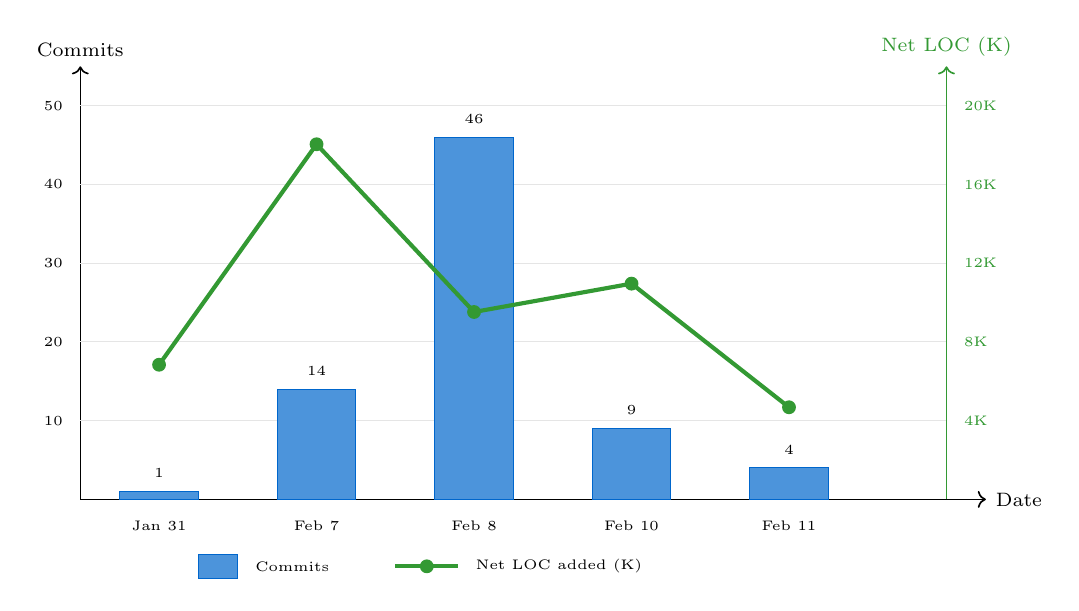
\begin{tikzpicture}[
  bar/.style={fill=extblue!70, draw=extblue, line width=0.4pt},
  addbar/.style={fill=webgreen!60, draw=webgreen!80, line width=0.4pt},
]
  % Axes
  \draw[->, line width=0.6pt] (0,0) -- (11.5,0) node[right, font=\scriptsize] {Date};
  \draw[->, line width=0.6pt] (0,0) -- (0,5.5) node[above, font=\scriptsize] {Commits};

  % Second y-axis (right) for LOC
  \draw[->, line width=0.6pt, webgreen!80] (11,0) -- (11,5.5) node[above, font=\scriptsize, webgreen!80] {Net LOC (K)};

  % Grid lines
  \foreach \y in {1,2,3,4,5} {
    \draw[gray!20, line width=0.3pt] (0,\y) -- (11,\y);
  }

  % Y-axis ticks (left: commits)
  \foreach \y/\lab in {1/10, 2/20, 3/30, 4/40, 5/50} {
    \node[font=\tiny, anchor=east] at (-0.1, \y) {\lab};
  }

  % Y-axis ticks (right: net LOC in thousands)
  \foreach \y/\lab in {1/4, 2/8, 3/12, 4/16, 5/20} {
    \node[font=\tiny, anchor=west, webgreen!80] at (11.1, \y) {\lab K};
  }

  % Commit bars (scaled: commits / 10)
  % Jan 31: 1 commit
  \draw[bar] (0.5,0) rectangle (1.5, 0.1);
  \node[font=\tiny, anchor=south] at (1.0, 0.15) {1};

  % Feb 7: 14 commits
  \draw[bar] (2.5,0) rectangle (3.5, 1.4);
  \node[font=\tiny, anchor=south] at (3.0, 1.45) {14};

  % Feb 8: 46 commits
  \draw[bar] (4.5,0) rectangle (5.5, 4.6);
  \node[font=\tiny, anchor=south] at (5.0, 4.65) {46};

  % Feb 10: 9 commits
  \draw[bar] (6.5,0) rectangle (7.5, 0.9);
  \node[font=\tiny, anchor=south] at (7.0, 0.95) {9};

  % Feb 11: 4 commits
  \draw[bar] (8.5,0) rectangle (9.5, 0.4);
  \node[font=\tiny, anchor=south] at (9.0, 0.45) {4};

  % Net LOC line (additions - deletions, scaled: /4000)
  % Jan 31: +6848 = 1.71
  % Feb 7: +18059 = 4.51
  % Feb 8: +9511 = 2.38
  % Feb 10: +10974 = 2.74
  % Feb 11: +4680 = 1.17
  \draw[addbar, line width=1.5pt, fill=none, draw=webgreen!80]
    (1.0, 1.71) -- (3.0, 4.51) -- (5.0, 2.38) -- (7.0, 2.74) -- (9.0, 1.17);
  \foreach \x/\y in {1.0/1.71, 3.0/4.51, 5.0/2.38, 7.0/2.74, 9.0/1.17} {
    \fill[webgreen!80] (\x,\y) circle (2.5pt);
  }

  % X-axis labels
  \node[font=\tiny, anchor=north] at (1.0, -0.15) {Jan 31};
  \node[font=\tiny, anchor=north] at (3.0, -0.15) {Feb 7};
  \node[font=\tiny, anchor=north] at (5.0, -0.15) {Feb 8};
  \node[font=\tiny, anchor=north] at (7.0, -0.15) {Feb 10};
  \node[font=\tiny, anchor=north] at (9.0, -0.15) {Feb 11};

  % Legend
  \draw[bar] (1.5, -1.0) rectangle (2.0, -0.7);
  \node[font=\tiny, anchor=west] at (2.1, -0.85) {Commits};
  \draw[webgreen!80, line width=1.5pt] (4.0, -0.85) -- (4.8, -0.85);
  \fill[webgreen!80] (4.4, -0.85) circle (2.5pt);
  \node[font=\tiny, anchor=west] at (4.9, -0.85) {Net LOC added (K)};

\end{tikzpicture}
\caption{Daily commit activity (blue bars, left axis) and net lines of code added (green line, right axis) across the five active development days. February~8 was the most intensive session with 46 commits, while February~7 produced the highest net code additions (+18K~lines) as the web platform and extension foundations were built simultaneously.}
\label{fig:commits}
\end{figure}


\subsection{Codebase composition}

Table~\ref{tab:codebase} breaks down the current codebase by component.

\begin{table}[htp!]
\centering
\small
\begin{tabular}{|l|r|r|}
\hline
\textbf{Component} & \textbf{LOC} & \textbf{Files} \\
\hline
VS~Code Extension (source) & 4,986 & 12 \\
\hline
Extension tests & 2,663 & 10 \\
\hline
Web platform library (\texttt{lib/}) & 3,243 & 10 \\
\hline
Library tests & 899 & 4 \\
\hline
React components & 4,811 & 22 \\
\hline
App pages (\texttt{app/}) & 3,675 & 28 \\
\hline
Content (JSON) & 1,795 & 5 \\
\hline
\textbf{Total TypeScript/TSX} & \textbf{20,164} & -- \\
\hline
\end{tabular}
\caption{Codebase composition by component (v0.4.0). Test code represents 17.7\% of the total codebase (3,562 out of 20,164 LOC), indicating substantial testing investment.}
\label{tab:codebase}
\end{table}

\subsection{Test distribution}

Figure~\ref{fig:testdist} visualizes the distribution of the 272 test cases across the 14 test files.

\begin{figure}[htp!]
\centering
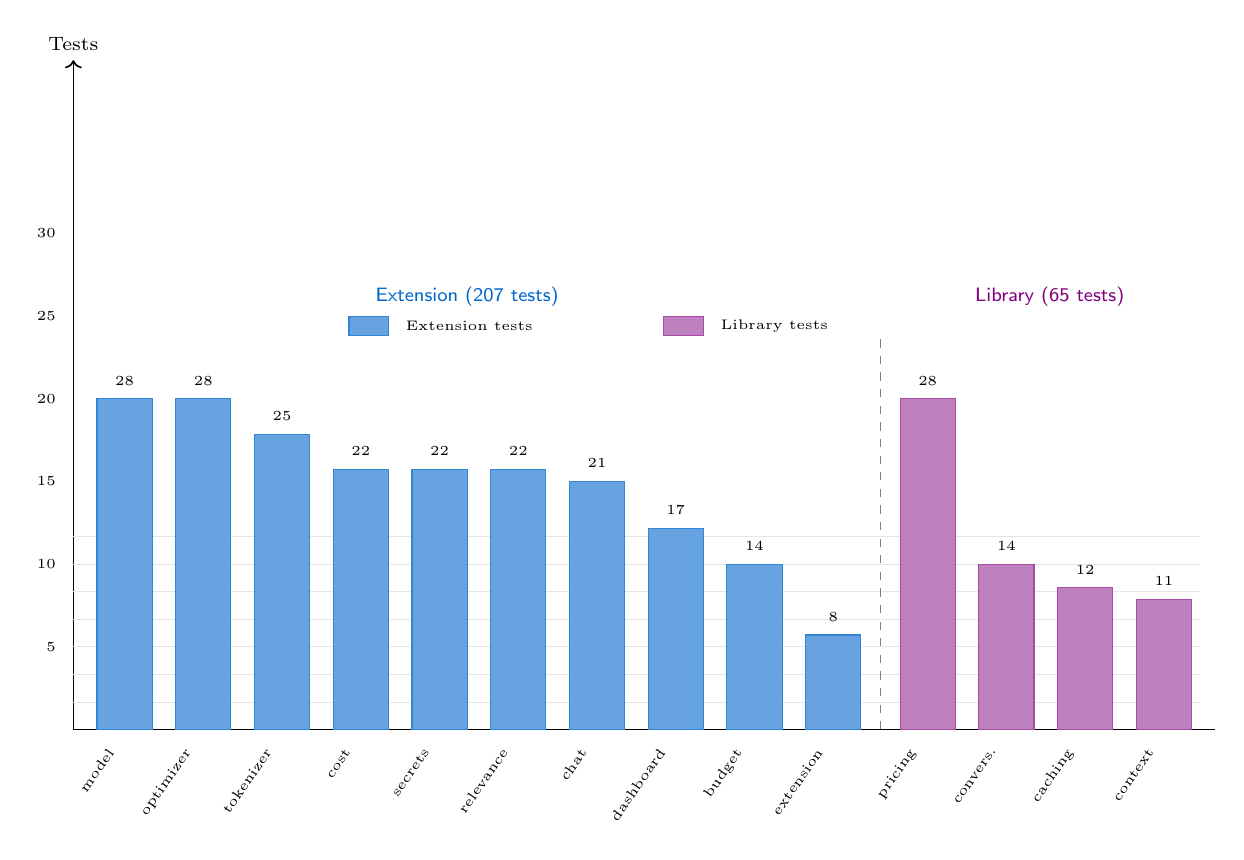
\begin{tikzpicture}[
  extbar/.style={fill=extblue!60, draw=extblue!80, line width=0.4pt},
  libbar/.style={fill=catpurple!50, draw=catpurple!70, line width=0.4pt},
]
  % Axes
  \draw[->, line width=0.6pt] (0,0) -- (0,8.5) node[above, font=\scriptsize] {Tests};
  \draw[line width=0.6pt] (0,0) -- (14.5,0);

  % Grid lines
  \foreach \y in {1,...,7} {
    \draw[gray!20, line width=0.3pt] (0,\y*0.35) -- (14.3,\y*0.35);
  }

  % Y-axis ticks (scaled: value * 0.25)
  \foreach \y/\lab in {0.7/5, 1.4/10, 2.1/15, 2.8/20, 3.5/25, 4.2/30} {
    \node[font=\tiny, anchor=east] at (-0.1, \y*1.5) {\lab};
  }

  % Extension test bars (10 files) — scaled by *0.25
  % modelProfiles: 28, contextOptimizer: 28, tokenizerService: 25,
  % costEstimator: 22, secretScanner: 22, tabRelevanceScorer: 22,
  % chatParticipant: 21, dashboardProvider: 17, tokenBudgetEstimator: 14, extension: 8

  \draw[extbar] (0.3,0) rectangle (1.0, 4.2);   % modelProfiles: 28
  \node[font=\tiny, anchor=south] at (0.65, 4.25) {28};

  \draw[extbar] (1.3,0) rectangle (2.0, 4.2);   % contextOptimizer: 28
  \node[font=\tiny, anchor=south] at (1.65, 4.25) {28};

  \draw[extbar] (2.3,0) rectangle (3.0, 3.75);   % tokenizerService: 25
  \node[font=\tiny, anchor=south] at (2.65, 3.8) {25};

  \draw[extbar] (3.3,0) rectangle (4.0, 3.3);   % costEstimator: 22
  \node[font=\tiny, anchor=south] at (3.65, 3.35) {22};

  \draw[extbar] (4.3,0) rectangle (5.0, 3.3);   % secretScanner: 22
  \node[font=\tiny, anchor=south] at (4.65, 3.35) {22};

  \draw[extbar] (5.3,0) rectangle (6.0, 3.3);   % tabRelevanceScorer: 22
  \node[font=\tiny, anchor=south] at (5.65, 3.35) {22};

  \draw[extbar] (6.3,0) rectangle (7.0, 3.15);   % chatParticipant: 21
  \node[font=\tiny, anchor=south] at (6.65, 3.2) {21};

  \draw[extbar] (7.3,0) rectangle (8.0, 2.55);   % dashboardProvider: 17
  \node[font=\tiny, anchor=south] at (7.65, 2.6) {17};

  \draw[extbar] (8.3,0) rectangle (9.0, 2.1);   % tokenBudgetEstimator: 14
  \node[font=\tiny, anchor=south] at (8.65, 2.15) {14};

  \draw[extbar] (9.3,0) rectangle (10.0, 1.2);   % extension: 8
  \node[font=\tiny, anchor=south] at (9.65, 1.25) {8};

  % Library test bars (4 files)
  \draw[libbar] (10.5,0) rectangle (11.2, 4.2);   % pricing: 28
  \node[font=\tiny, anchor=south] at (10.85, 4.25) {28};

  \draw[libbar] (11.5,0) rectangle (12.2, 2.1);   % conversation: 14
  \node[font=\tiny, anchor=south] at (11.85, 2.15) {14};

  \draw[libbar] (12.5,0) rectangle (13.2, 1.8);   % caching: 12
  \node[font=\tiny, anchor=south] at (12.85, 1.85) {12};

  \draw[libbar] (13.5,0) rectangle (14.2, 1.65);   % context: 11
  \node[font=\tiny, anchor=south] at (13.85, 1.7) {11};

  % Separator line
  \draw[gray, dashed, line width=0.4pt] (10.25, 0) -- (10.25, 5.0);

  % X-axis labels (rotated)
  \foreach \x/\lab in {
    0.65/{\rotatebox{55}{\tiny model}},
    1.65/{\rotatebox{55}{\tiny optimizer}},
    2.65/{\rotatebox{55}{\tiny tokenizer}},
    3.65/{\rotatebox{55}{\tiny cost}},
    4.65/{\rotatebox{55}{\tiny secrets}},
    5.65/{\rotatebox{55}{\tiny relevance}},
    6.65/{\rotatebox{55}{\tiny chat}},
    7.65/{\rotatebox{55}{\tiny dashboard}},
    8.65/{\rotatebox{55}{\tiny budget}},
    9.65/{\rotatebox{55}{\tiny extension}},
    10.85/{\rotatebox{55}{\tiny pricing}},
    11.85/{\rotatebox{55}{\tiny convers.}},
    12.85/{\rotatebox{55}{\tiny caching}},
    13.85/{\rotatebox{55}{\tiny context}}
  } {
    \node[anchor=north east] at (\x, -0.1) {\lab};
  }

  % Labels
  \node[font=\scriptsize\sffamily, extblue] at (5.0, 5.5) {Extension (207 tests)};
  \node[font=\scriptsize\sffamily, catpurple] at (12.4, 5.5) {Library (65 tests)};

  % Legend
  \draw[extbar] (3.5, 5.0) rectangle (4.0, 5.25);
  \node[font=\tiny, anchor=west] at (4.1, 5.125) {Extension tests};
  \draw[libbar] (7.5, 5.0) rectangle (8.0, 5.25);
  \node[font=\tiny, anchor=west] at (8.1, 5.125) {Library tests};

\end{tikzpicture}
\caption{Distribution of 272 test cases across 14 test files. Extension tests (blue, left of dashed line) cover 10 modules; library tests (purple, right) cover 4 shared modules. The most-tested modules are Model Profiles, Context Optimizer, and Pricing Engine (28 tests each), reflecting their critical role in the toolkit.}
\label{fig:testdist}
\end{figure}


\subsection{AI-assisted development sessions}

%% ── EDIT NOTE FOR VAHID ──
%% The session details below are estimated from our conversation
%% history and git timestamps. Update with your actual records
%% if you tracked hours more precisely.
%%
%% Token sizes: Each session with Claude involved substantial context.
%% Typical session context: 30K-80K tokens input per exchange,
%% with the later paper sessions reaching 100K+ tokens as the
%% full paper was loaded for review.
%%
%% If you have Copilot usage stats from VS Code or Claude usage
%% from your Anthropic account, add those exact numbers.
%%

Table~\ref{tab:sessions} summarizes the AI-assisted development sessions. All sessions used GitHub Copilot (VS~Code) for inline code completion and Claude (Anthropic) for interactive pair-programming via chat. The AI tools accelerated implementation; all design decisions, architectural choices, and mathematical formulations were made by the authors.

\begin{table}[htp!]
\centering
\small
\begin{tabular}{|r|l|p{5.5cm}|r|}
\hline
\textbf{\#} & \textbf{Date} & \textbf{Focus} & \textbf{Commits} \\
\hline
1 & Jan 31 & Project scaffold (Next.js~16, initial structure) & 1 \\
\hline
2 & Feb 7 & Web platform foundation: pricing lib, calculators, wiki, dictionary, catalog, homepage, responsive design & 14 \\
\hline
3 & Feb 8 & Extension v0.2.0--v0.2.6: core monitor, tokenizer service, chat participant (14 commands), dashboard webview, model profiles, relevance scorer; web: learn course, about page, marketplace publishing & 46 \\
\hline
4 & Feb 10 & Extension v0.2.7--v0.3.0: dashboard theme fixes, model profile updates, initial test suite (148~tests), UI polish, Marketplace sync & 9 \\
\hline
5 & Feb 11 & Extension v0.4.0: secret scanner (381~LOC), cost estimator (257~LOC), context optimizer (473~LOC), 80+~new tests, homepage cleanup, paper update & 4 \\
\hline
\multicolumn{3}{|l|}{\textbf{Total}} & \textbf{74} \\
\hline
\end{tabular}
\caption{AI-assisted development sessions. Each session used GitHub Copilot for inline completions and Claude for interactive pair-programming. Estimated total active development time: $\sim$60~hours across 5~days.}
\label{tab:sessions}
\end{table}

The cumulative Git statistics across all 74 commits are: \textbf{+60,247} insertions and \textbf{--10,175} deletions, yielding a net codebase of $\sim$50K lines (including content, configuration, and documentation). The current TypeScript/TSX codebase totals \textbf{20,164~LOC} (Table~\ref{tab:codebase}), indicating that approximately 60\% of all code written was later refactored or replaced---a natural consequence of the iterative, AI-assisted development workflow where rapid prototyping is followed by manual refinement.

%% ── SUGGESTION: Add context token usage if you have it ──
%% If you have access to your Anthropic API usage dashboard or
%% Claude conversation history, add a paragraph like:
%%
%% "Across the five development sessions, the AI-assisted coding
%% consumed approximately [X] million input tokens and [Y] million
%% output tokens via Claude, plus an estimated [Z] million tokens
%% via GitHub Copilot inline completions. The later sessions
%% (paper review, test generation) involved larger context windows
%% as the full codebase and paper were loaded for analysis."
%%
%% This is meta-interesting for a paper about token economics ---
%% you're eating your own dog food.
%%

\section{Glossary of Key Terms}
\label{app:glossary}

%% ── EDIT NOTE: These definitions are derived from the dashboard,
%% chat participant, optimizer, and dictionary. Add/remove as needed.
%% The full 41-term dictionary is at tokalator.wiki/dictionary.
%%

Table~\ref{tab:glossary} defines the key technical terms used in Tokalator's dashboard, chat interface, and optimization engine. These terms map abstract context engineering concepts to actionable indicators visible in the developer's IDE.

\begin{table}[htp!]
\centering
\small
\begin{tabular}{|l|p{9.5cm}|}
\hline
\textbf{Term} & \textbf{Definition} \\
\hline
\multicolumn{2}{|l|}{\textit{Context Management}} \\
\hline
Context Window & The maximum number of tokens an LLM can process in a single request, including input and output. Ranges from 128K to 1M tokens as of early 2026. \\
\hline
Context Rot & Progressive degradation of model performance as input length increases, even on simple tasks~\cite{hong2025contextrot}. Tokalator warns at provider-specific rot thresholds. \\
\hline
Rot Threshold & The turn count or token count at which context rot begins to degrade output quality. Default: 20 turns. \\
\hline
Context Health & A tri-state indicator (\texttt{healthy}, \texttt{warning}, \texttt{critical}) reflecting the overall quality of the developer's context window based on budget utilization, secret exposure, and distractor count. \\
\hline
Distractors & Open files with low relevance scores ($R < 0.3$) that consume context budget without contributing to the current task. Analogous to noise in signal processing. \\
\hline
Compaction Point & The estimated turn number at which cumulative context will exceed the rot threshold, triggering a recommendation to summarize or restart the conversation. \\
\hline
Next Turn Preview & A projection of the total token count after the next conversational turn, helping developers decide whether to send a message or compact first. \\
\hline
\multicolumn{2}{|l|}{\textit{Token Economics}} \\
\hline
Budget Level & A tri-state classification of context utilization: \texttt{low} ($<50\%$), \texttt{medium} (50--80\%), \texttt{high} ($>80\%$). Displayed as a colored badge in the dashboard. \\
\hline
Budget Breakdown & The decomposition of total estimated tokens into five components: files, system prompt, instructions, conversation history, and output reservation. \\
\hline
Output Reservation & Tokens reserved for the model's response (default: 4,000). Not sent as input but must be subtracted from the available context window. \\
\hline
System Overhead & Hidden tokens injected by the AI assistant's framework (system prompts, tool definitions, internal formatting) that consume context budget invisibly. \\
\hline
Input Growth Rate & The rate at which per-turn input tokens increase across a conversation, driven by conversation history accumulation. \\
\hline
\multicolumn{2}{|l|}{\textit{Relevance \& Scoring}} \\
\hline
Relevance Score ($R$) & A value in $[0, 1]$ assigned to each open tab (Equation~2), computed from five weighted signals: language match, import relationship, path similarity, edit recency, and diagnostics. \\
\hline
Optimization Score & A value in $[0, 100]$ produced by the nine-analyzer pipeline, reflecting overall context health. Verdicts: \texttt{great} ($\geq 85$), \texttt{good} (70--84), \texttt{fair} (50--69), \texttt{poor} ($<50$). \\
\hline
Pinned Files & Files explicitly marked by the developer to always receive $R = 1.0$, overriding algorithmic scoring. Persisted across VS~Code sessions. \\
\hline
\multicolumn{2}{|l|}{\textit{Caching \& Cost}} \\
\hline
Blended Cost & The weighted average of cached and uncached per-token rates, reflecting the effective input cost when prompt caching is active: $c_{\text{blend}} = r \cdot c_r + (1 - r) \cdot c_{\text{in}}$, where $r$ is the cache hit ratio. \\
\hline
Cacheable Tokens & Tokens in the stable prefix (system prompt, instructions, pinned files) eligible for prompt caching across turns. \\
\hline
Volatile Tokens & Tokens that change between turns (conversation history, edited file content) and cannot benefit from prompt caching. \\
\hline
Cache Hit Ratio & The estimated fraction of cacheable tokens that will be served from cache on a given turn. Provider-dependent: Anthropic $\approx 0.85$, OpenAI $\approx 0.50$, Google $\approx 0.70$. \\
\hline
Break-Even Point ($n^*$) & The number of prompt reuses after which caching becomes cheaper than re-sending tokens uncached (Equation~4). \\
\hline
Session Projection & Extrapolation of per-turn costs to session (10/25/50 turns), daily (8 sessions), and monthly (22 working days) estimates. \\
\hline
\multicolumn{2}{|l|}{\textit{Security}} \\
\hline
Secrets Guard & A real-time scanner that detects exposed credentials (API keys, tokens, connection strings) in open files before they enter the AI assistant's context window. \\
\hline
Sensitive File & A file whose name matches known credential patterns (\texttt{.env}, \texttt{.pem}, \texttt{id\_rsa}, etc.) and is flagged regardless of content. \\
\hline
Severity Tiers & Classification of detected secrets: \texttt{critical} (cloud provider keys, private keys), \texttt{high} (API keys, database URLs), \texttt{warning} (generic patterns, internal IPs). \\
\hline
\end{tabular}
\caption{Glossary of key technical terms used in the Tokalator dashboard, chat interface, and optimization engine. These terms are also available in the online dictionary at \url{https://tokalator.wiki/dictionary}, which defines 41 terms across seven categories.}
\label{tab:glossary}
\end{table}

%% ═══════════════════════════════════════════════════════════════════
%% REFERENCES (17 entries)
%% ═══════════════════════════════════════════════════════════════════
%% REVIEW: 17 references is reasonable for a tool paper. However:
%% - [1] Bergemann et al. is "Working Paper" — is it published yet?
%%   If accepted, update with journal/venue.
%% - [8]-[12] use inconsistent formatting: some have year in parens,
%%   some don't. Standardize to BibTeX elsarticle style.
%% - [13]-[16] are blog posts / GitHub repos. SoftwareX allows these
%%   but mark them clearly as "[Online]" or "Technical Report."
%% - Consider adding the Anthropic pricing/caching refs [2,3] into
%%   the body text more — they're cited but feel orphaned.
\begin{thebibliography}{00}

\bibitem{bergemann2025economics}
D.~Bergemann, A.~Bonatti, A.~Smolin,
The Economics of Large Language Models,
Working Paper, 2025. Available at SSRN.

\bibitem{anthropic2026pricing}
Anthropic,
Claude API Pricing,
\url{https://docs.anthropic.com/en/docs/about-claude/pricing}, February 2026.

\bibitem{anthropic2025caching}
Anthropic,
Prompt Caching,
\url{https://docs.anthropic.com/en/docs/build-with-claude/prompt-caching}, 2025.

\bibitem{openai2026pricing}
OpenAI,
API Pricing,
\url{https://openai.com/api/pricing/}, February 2026.

\bibitem{google2026pricing}
Google,
Gemini API Pricing,
\url{https://ai.google.dev/pricing}, February 2026.

\bibitem{sennrich2016bpe}
R.~Sennrich, B.~Haddow, A.~Birch,
Neural Machine Translation of Rare Words with Subword Units,
in: Proceedings of ACL, 2016.

\bibitem{vscode2026api}
Microsoft,
VS~Code Extension API,
\url{https://code.visualstudio.com/api}, 2026.


\bibitem{aubakirova2025state} Aubakirova, M., et al. (2025). \textit{State of AI: An Empirical 100 Trillion Token Study with OpenRouter}.

\bibitem{burnham2025context} Burnham, G. \& Adamczewski, T. (2025). \textit{Context Engineering for AI Agents: Lessons from Building Real-World Systems}. Anthropic Research Blog.

\bibitem{emberson2025length} Emberson, L., et al. (2025). \textit{LLM responses to benchmark questions are getting longer over time}. Epoch AI.
\bibitem{erdil2025pareto} Erdil, E. (2025). \textit{Pareto Frontiers of Language Model Inference Economics}. Epoch AI.
\bibitem{cottier2025price} Cottier, B., et al. (2025). \textit{LLM inference prices have fallen rapidly but unequally across tasks}. Epoch AI.
\bibitem{yotta2026econ} Yotta Labs. (2026). \textit{The Economics of LLM Inference: Beyond Cost Per Token}.

\bibitem{hong2025contextrot}
K.~Hong, A.~Troynikov, J.~Huber,
Context Rot: How Increasing Input Tokens Impacts LLM Performance,
Chroma Technical Report, July 2025.
\url{https://research.trychroma.com/context-rot}

\bibitem{anthropic2025contexteng}
P.~Rajasekaran, E.~Dixon, C.~Ryan, J.~Hadfield,
Effective Context Engineering for AI Agents,
Anthropic Engineering Blog, September 2025.
\url{https://www.anthropic.com/engineering/effective-context-engineering-for-ai-agents}

\bibitem{navid2025compaction}
P.~Navid,
Automatic Context Compaction,
Claude Cookbook, Anthropic, November 2025.
\url{https://platform.claude.com/cookbook/tool-use-automatic-context-compaction}

\bibitem{zhu2025onecontext}
J.~Zhu, et al.,
OneContext: An Agent Self-Managed Context Layer,
GitHub, 2025.
\url{https://github.com/TheAgentContextLab/OneContext}

\end{thebibliography}

\end{document}
